\documentclass[11pt,letterpaper]{article}

% Build steps (from this folder):
% 1) pdflatex Module2.tex
% 2) makeglossaries Module2
% 3) pdflatex Module2.tex
% 4) pdflatex Module2.tex

% ── Packages ──────────────────────────────────────────────────
\usepackage[margin=1in]{geometry}
\usepackage{titlesec}
\usepackage{enumitem}
\usepackage{booktabs}
\usepackage{tabularx}
\usepackage{graphicx}
\usepackage{xcolor}
\usepackage{hyperref}
\usepackage{fancyhdr}
\usepackage{amsmath}
\usepackage{tcolorbox}
\usepackage{multicol}
\usepackage{caption}
\usepackage{tikz}
\usepackage{listings}
\usepackage[acronym,toc,nopostdot]{glossaries}
\usetikzlibrary{shapes.geometric, arrows.meta, positioning, fit, calc, decorations.pathreplacing}
\makenoidxglossaries%
% Shared acronym macro container for EE800/820 lesson plan modules.
% Usage: type \IDE, \FPGA, \UART, etc. First use is expanded; later uses show acronym only.
% Requires in each document preamble:
%   \usepackage[acronym,toc]{glossaries}
%   \makeglossaries
%   % Shared acronym macro container for EE800/820 lesson plan modules.
% Usage: type \IDE, \FPGA, \UART, etc. First use is expanded; later uses show acronym only.
% Requires in each document preamble:
%   \usepackage[acronym,toc]{glossaries}
%   \makeglossaries
%   % Shared acronym macro container for EE800/820 lesson plan modules.
% Usage: type \IDE, \FPGA, \UART, etc. First use is expanded; later uses show acronym only.
% Requires in each document preamble:
%   \usepackage[acronym,toc]{glossaries}
%   \makeglossaries
%   \input{../glossary}
% Print used acronyms near end of document:
%   \printglossary[type=\acronymtype,title={Acronyms Used}]

% Acronym definitions (only used entries appear in the printed glossary).
\newacronym{ask}{ASK}{Amplitude Shift Keying}
\newacronym{bga}{BGA}{Ball Grid Array}
\newacronym{bom}{BOM}{Bill of Materials}
\newacronym{bram}{BRAM}{Block Random Access Memory}
\newacronym{crc}{CRC}{Cyclic Redundancy Check}
\newacronym{css}{CSS}{Chirp Spread Spectrum}
\newacronym{dma}{DMA}{Direct Memory Access}
\newacronym{dsp}{DSP}{Digital Signal Processing}
\newacronym{eda}{EDA}{Exploratory Data Analysis}
\newacronym{fifo}{FIFO}{First In, First Out}
\newacronym{fpga}{FPGA}{Field-Programmable Gate Array}
\newacronym{fsk}{FSK}{Frequency Shift Keying}
\newacronym{fsm}{FSM}{Finite State Machine}
\newacronym{gpio}{GPIO}{General-Purpose Input/Output}
\newacronym{hal}{HAL}{Hardware Abstraction Layer}
\newacronym{i2c}{I\textsuperscript{2}C}{Inter-Integrated Circuit}
\newacronym{ide}{IDE}{Integrated Development Environment}
\newacronym{ila}{ILA}{Integrated Logic Analyzer}
\newacronym{ism}{ISM}{Industrial, Scientific, and Medical}
\newacronym{isr}{ISR}{Interrupt Service Routine}
\newacronym{lut}{LUT}{Look-Up Table}
\newacronym{mcu}{MCU}{Microcontroller Unit}
\newacronym{ml}{ML}{Machine Learning}
\newacronym{ook}{OOK}{On-Off Keying}
\newacronym{per}{PER}{Packet Error Rate}
\newacronym{rf}{RF}{Radio Frequency}
\newacronym{rssi}{RSSI}{Received Signal Strength Indicator}
\newacronym{rtl}{RTL}{Register-Transfer Level}
\newacronym{snr}{SNR}{Signal-to-Noise Ratio}
\newacronym{spi}{SPI}{Serial Peripheral Interface}
\newacronym{uart}{UART}{Universal Asynchronous Receiver/Transmitter}
\newacronym{vhdl}{VHDL}{VHSIC Hardware Description Language}

% Convenience wrappers so you can type \IDE, \RF, etc.
\providecommand{\ASK}{\gls{ask}}
\providecommand{\BGA}{\gls{bga}}
\providecommand{\BOM}{\gls{bom}}
\providecommand{\BRAM}{\gls{bram}}
\providecommand{\CRC}{\gls{crc}}
\providecommand{\CSS}{\gls{css}}
\providecommand{\DMA}{\gls{dma}}
\providecommand{\DSP}{\gls{dsp}}
\providecommand{\EDA}{\gls{eda}}
\providecommand{\FIFO}{\gls{fifo}}
\providecommand{\FPGA}{\gls{fpga}}
\providecommand{\FSK}{\gls{fsk}}
\providecommand{\FSM}{\gls{fsm}}
\providecommand{\GPIO}{\gls{gpio}}
\providecommand{\HAL}{\gls{hal}}
\providecommand{\IIC}{\gls{i2c}}
\providecommand{\IDE}{\gls{ide}}
\providecommand{\ILA}{\gls{ila}}
\providecommand{\ISM}{\gls{ism}}
\providecommand{\ISR}{\gls{isr}}
\providecommand{\LUT}{\gls{lut}}
\providecommand{\MCU}{\gls{mcu}}
\providecommand{\ML}{\gls{ml}}
\providecommand{\OOK}{\gls{ook}}
\providecommand{\PER}{\gls{per}}
\providecommand{\RF}{\gls{rf}}
\providecommand{\RSSI}{\gls{rssi}}
\providecommand{\RTL}{\gls{rtl}}
\providecommand{\SNR}{\gls{snr}}
\providecommand{\SPI}{\gls{spi}}
\providecommand{\UART}{\gls{uart}}
\providecommand{\VHDL}{\gls{vhdl}}


% Print used acronyms near end of document:
%   \printglossary[type=\acronymtype,title={Acronyms Used}]

% Acronym definitions (only used entries appear in the printed glossary).
\newacronym{ask}{ASK}{Amplitude Shift Keying}
\newacronym{bga}{BGA}{Ball Grid Array}
\newacronym{bom}{BOM}{Bill of Materials}
\newacronym{bram}{BRAM}{Block Random Access Memory}
\newacronym{crc}{CRC}{Cyclic Redundancy Check}
\newacronym{css}{CSS}{Chirp Spread Spectrum}
\newacronym{dma}{DMA}{Direct Memory Access}
\newacronym{dsp}{DSP}{Digital Signal Processing}
\newacronym{eda}{EDA}{Exploratory Data Analysis}
\newacronym{fifo}{FIFO}{First In, First Out}
\newacronym{fpga}{FPGA}{Field-Programmable Gate Array}
\newacronym{fsk}{FSK}{Frequency Shift Keying}
\newacronym{fsm}{FSM}{Finite State Machine}
\newacronym{gpio}{GPIO}{General-Purpose Input/Output}
\newacronym{hal}{HAL}{Hardware Abstraction Layer}
\newacronym{i2c}{I\textsuperscript{2}C}{Inter-Integrated Circuit}
\newacronym{ide}{IDE}{Integrated Development Environment}
\newacronym{ila}{ILA}{Integrated Logic Analyzer}
\newacronym{ism}{ISM}{Industrial, Scientific, and Medical}
\newacronym{isr}{ISR}{Interrupt Service Routine}
\newacronym{lut}{LUT}{Look-Up Table}
\newacronym{mcu}{MCU}{Microcontroller Unit}
\newacronym{ml}{ML}{Machine Learning}
\newacronym{ook}{OOK}{On-Off Keying}
\newacronym{per}{PER}{Packet Error Rate}
\newacronym{rf}{RF}{Radio Frequency}
\newacronym{rssi}{RSSI}{Received Signal Strength Indicator}
\newacronym{rtl}{RTL}{Register-Transfer Level}
\newacronym{snr}{SNR}{Signal-to-Noise Ratio}
\newacronym{spi}{SPI}{Serial Peripheral Interface}
\newacronym{uart}{UART}{Universal Asynchronous Receiver/Transmitter}
\newacronym{vhdl}{VHDL}{VHSIC Hardware Description Language}

% Convenience wrappers so you can type \IDE, \RF, etc.
\providecommand{\ASK}{\gls{ask}}
\providecommand{\BGA}{\gls{bga}}
\providecommand{\BOM}{\gls{bom}}
\providecommand{\BRAM}{\gls{bram}}
\providecommand{\CRC}{\gls{crc}}
\providecommand{\CSS}{\gls{css}}
\providecommand{\DMA}{\gls{dma}}
\providecommand{\DSP}{\gls{dsp}}
\providecommand{\EDA}{\gls{eda}}
\providecommand{\FIFO}{\gls{fifo}}
\providecommand{\FPGA}{\gls{fpga}}
\providecommand{\FSK}{\gls{fsk}}
\providecommand{\FSM}{\gls{fsm}}
\providecommand{\GPIO}{\gls{gpio}}
\providecommand{\HAL}{\gls{hal}}
\providecommand{\IIC}{\gls{i2c}}
\providecommand{\IDE}{\gls{ide}}
\providecommand{\ILA}{\gls{ila}}
\providecommand{\ISM}{\gls{ism}}
\providecommand{\ISR}{\gls{isr}}
\providecommand{\LUT}{\gls{lut}}
\providecommand{\MCU}{\gls{mcu}}
\providecommand{\ML}{\gls{ml}}
\providecommand{\OOK}{\gls{ook}}
\providecommand{\PER}{\gls{per}}
\providecommand{\RF}{\gls{rf}}
\providecommand{\RSSI}{\gls{rssi}}
\providecommand{\RTL}{\gls{rtl}}
\providecommand{\SNR}{\gls{snr}}
\providecommand{\SPI}{\gls{spi}}
\providecommand{\UART}{\gls{uart}}
\providecommand{\VHDL}{\gls{vhdl}}


% Print used acronyms near end of document:
%   \printglossary[type=\acronymtype,title={Acronyms Used}]

% Acronym definitions (only used entries appear in the printed glossary).
\newacronym{ask}{ASK}{Amplitude Shift Keying}
\newacronym{bga}{BGA}{Ball Grid Array}
\newacronym{bom}{BOM}{Bill of Materials}
\newacronym{bram}{BRAM}{Block Random Access Memory}
\newacronym{crc}{CRC}{Cyclic Redundancy Check}
\newacronym{css}{CSS}{Chirp Spread Spectrum}
\newacronym{dma}{DMA}{Direct Memory Access}
\newacronym{dsp}{DSP}{Digital Signal Processing}
\newacronym{eda}{EDA}{Exploratory Data Analysis}
\newacronym{fifo}{FIFO}{First In, First Out}
\newacronym{fpga}{FPGA}{Field-Programmable Gate Array}
\newacronym{fsk}{FSK}{Frequency Shift Keying}
\newacronym{fsm}{FSM}{Finite State Machine}
\newacronym{gpio}{GPIO}{General-Purpose Input/Output}
\newacronym{hal}{HAL}{Hardware Abstraction Layer}
\newacronym{i2c}{I\textsuperscript{2}C}{Inter-Integrated Circuit}
\newacronym{ide}{IDE}{Integrated Development Environment}
\newacronym{ila}{ILA}{Integrated Logic Analyzer}
\newacronym{ism}{ISM}{Industrial, Scientific, and Medical}
\newacronym{isr}{ISR}{Interrupt Service Routine}
\newacronym{lut}{LUT}{Look-Up Table}
\newacronym{mcu}{MCU}{Microcontroller Unit}
\newacronym{ml}{ML}{Machine Learning}
\newacronym{ook}{OOK}{On-Off Keying}
\newacronym{per}{PER}{Packet Error Rate}
\newacronym{rf}{RF}{Radio Frequency}
\newacronym{rssi}{RSSI}{Received Signal Strength Indicator}
\newacronym{rtl}{RTL}{Register-Transfer Level}
\newacronym{snr}{SNR}{Signal-to-Noise Ratio}
\newacronym{spi}{SPI}{Serial Peripheral Interface}
\newacronym{uart}{UART}{Universal Asynchronous Receiver/Transmitter}
\newacronym{vhdl}{VHDL}{VHSIC Hardware Description Language}

% Convenience wrappers so you can type \IDE, \RF, etc.
\providecommand{\ASK}{\gls{ask}}
\providecommand{\BGA}{\gls{bga}}
\providecommand{\BOM}{\gls{bom}}
\providecommand{\BRAM}{\gls{bram}}
\providecommand{\CRC}{\gls{crc}}
\providecommand{\CSS}{\gls{css}}
\providecommand{\DMA}{\gls{dma}}
\providecommand{\DSP}{\gls{dsp}}
\providecommand{\EDA}{\gls{eda}}
\providecommand{\FIFO}{\gls{fifo}}
\providecommand{\FPGA}{\gls{fpga}}
\providecommand{\FSK}{\gls{fsk}}
\providecommand{\FSM}{\gls{fsm}}
\providecommand{\GPIO}{\gls{gpio}}
\providecommand{\HAL}{\gls{hal}}
\providecommand{\IIC}{\gls{i2c}}
\providecommand{\IDE}{\gls{ide}}
\providecommand{\ILA}{\gls{ila}}
\providecommand{\ISM}{\gls{ism}}
\providecommand{\ISR}{\gls{isr}}
\providecommand{\LUT}{\gls{lut}}
\providecommand{\MCU}{\gls{mcu}}
\providecommand{\ML}{\gls{ml}}
\providecommand{\OOK}{\gls{ook}}
\providecommand{\PER}{\gls{per}}
\providecommand{\RF}{\gls{rf}}
\providecommand{\RSSI}{\gls{rssi}}
\providecommand{\RTL}{\gls{rtl}}
\providecommand{\SNR}{\gls{snr}}
\providecommand{\SPI}{\gls{spi}}
\providecommand{\UART}{\gls{uart}}
\providecommand{\VHDL}{\gls{vhdl}}



% ── Colors ────────────────────────────────────────────────────
\definecolor{stevens}{RGB}{163,31,52}       % Stevens Red
\definecolor{darkgray}{RGB}{60,60,60}
\definecolor{lightgray}{RGB}{240,240,240}
\definecolor{accentblue}{RGB}{30,80,140}

% ── Hyperref Setup ────────────────────────────────────────────
\hypersetup{
	colorlinks=true,
	linkcolor=stevens,
	urlcolor=accentblue,
	citecolor=darkgray,
	plainpages=false
}

% ── Header / Footer ──────────────────────────────────────────
\pagestyle{fancy}
\fancyhf{}
\fancyhead[L]{\small\textcolor{darkgray}{Stevens Institute of Technology}}
\fancyhead[R]{\small\textcolor{darkgray}{Spring 2026}}
\fancyfoot[C]{\thepage}
\renewcommand{\headrulewidth}{0.4pt}

% ── Section Formatting ───────────────────────────────────────
\titleformat{\section}
{\Large\bfseries\color{stevens}}{\thesection}{1em}{}[\vspace{-0.5em}\rule{\textwidth}{0.4pt}]
\titleformat{\subsection}
{\large\bfseries\color{darkgray}}{\thesubsection}{1em}{}

% ── tcolorbox Styles ─────────────────────────────────────────
\tcbset{
	objective/.style={colback=lightgray, colframe=stevens,
		fonttitle=\bfseries, title=#1, boxrule=0.5pt, arc=2pt},
	infobox/.style={colback=blue!5, colframe=accentblue,
		fonttitle=\bfseries, title=#1, boxrule=0.5pt, arc=2pt},
	deliverable/.style={colback=green!5, colframe=green!40!black,
		fonttitle=\bfseries, title=#1, boxrule=0.5pt, arc=2pt},
	warning/.style={colback=red!5, colframe=stevens,
		fonttitle=\bfseries, title=#1, boxrule=0.5pt, arc=2pt}
}

% ── Listings Style ───────────────────────────────────────────
\lstset{
	basicstyle=\small\ttfamily,
	keywordstyle=\color{accentblue}\bfseries,
	commentstyle=\color{darkgray}\itshape,
	stringstyle=\color{stevens},
	numbers=left,
	numberstyle=\tiny\color{darkgray},
	numbersep=8pt,
	frame=single,
	framerule=0.4pt,
	rulecolor=\color{darkgray},
	backgroundcolor=\color{lightgray},
	breaklines=true,
	tabsize=2,
	showstringspaces=false,
	captionpos=b
}

% ══════════════════════════════════════════════════════════════
\begin{document}

	% ── Title Page ───────────────────────────────────────────────
	\pagenumbering{Alph}
	\begin{titlepage}
		\centering
		\vspace*{2cm}

		{\Huge\bfseries\color{stevens} Lesson Plan: Module~2\par}
		\vspace{0.5cm}
		{\LARGE\color{darkgray} Field-Programmable Gate Array (\FPGA{}) Register-Transfer Level (\RTL{}) Design, Signal Ingestion Pipeline,\\[4pt]
			and Simulation Verification\par}

		\vspace{1.5cm}
		\rule{0.6\textwidth}{1pt}
		\vspace{1.5cm}

		{\Large\textbf{An Educational Framework for\\[4pt]
				AI-Driven Signal Processing}\par}

		\vspace{1.5cm}

		\begin{tabular}{rl}
			\textbf{Student:}         & Jude Eschete \\
			\textbf{Project Advisor:} & Dr.\ Bernard Yett \\
			\textbf{Program:}         & M.S.\ Computer Engineering \\
			\textbf{Institution:}     & Stevens Institute of Technology \\
			\textbf{Date Range:}      & March 15 -- March 28, 2026 \\
		\end{tabular}

		\vspace{2cm}

		\begin{tcolorbox}[colback=lightgray, colframe=darkgray, width=0.85\textwidth, arc=2pt]
			\centering\small
			This document presents the lesson plan for the second module of the capstone project,
			covering the design and simulation of the Field-Programmable Gate Array-side signal processing pipeline on the
			Digilent Nexys A7-100T. Students implement Universal Asynchronous Receiver/Transmitter-based data ingestion, packet parsing
			with hardware Cyclic Redundancy Check verification, and a feature extraction datapath in VHSIC Hardware Description Language, then verify
			the complete pipeline through simulation testbenches driven by recorded DATA / ACK / PAUSE captures from
			the Module~1 cooperative-target / interceptor platform.
		\end{tcolorbox}

		\vfill
		{\small\textcolor{darkgray}{JEschete@stevens.edu}}
	\end{titlepage}

	% ── Table of Contents ────────────────────────────────────────
	\pagenumbering{roman}
	\tableofcontents
	\newpage
	\pagenumbering{arabic}

	% ══════════════════════════════════════════════════════════════
	\section{Module Overview}
	% ══════════════════════════════════════════════════════════════

	\begin{tcolorbox}[objective={Module 2 Learning Objectives}]
		Upon completion of this module, the student (or future learner following this curriculum) will be able to:
		\begin{enumerate}[label=\textbf{LO-\arabic*}]
			\item Implement a \UART{} receiver module in \VHDL{} that reliably captures asynchronous serial data at 115200~baud and interfaces with the \FPGA's 100~MHz system clock domain through proper synchronization techniques.
			\item Design and implement a packet parser state machine that detects frame delimiters, extracts fixed-length fields, and routes parsed data to downstream processing stages.
			\item Implement hardware \CRC{} verification (\CRC{}-8 for the interceptor forwarding frame, \CRC{}-16 for the embedded radio packet) and use the results to gate downstream processing, rejecting corrupted frames in real time.
			\item Architect a feature extraction datapath that transforms parsed packet fields into a structured feature vector suitable for the \ML{} classification pipeline in Module~4.
			\item Develop simulation testbenches in \VHDL{} that use recorded interceptor capture data from Module~1 (DATA / ACK / PAUSE traffic) as stimulus, verify functional correctness of each pipeline stage, and identify timing or resource issues before hardware deployment.
			\item Analyze \FPGA{} resource utilization (look-up tables (\LUT{}s), flip-flops, block random access memory (\BRAM{}), and digital signal processing (DSP) slices) and timing reports to make informed design trade-offs within the Artix-7 fabric constraints.
		\end{enumerate}
	\end{tcolorbox}

	\subsection{Context Within the Project}

	Module~2 builds directly on the hardware platform validated in Module~1. The \UART{} interface between the interceptor (Threat) STM32 microcontroller unit (\MCU{}) and the Nexys A7 \FPGA{}, characterized in Session~4, becomes the input to the \RTL{} processing pipeline developed here. The 32-byte radio packet format (Table~4 in Module~1, shared by DATA, ACK, and PAUSE) and the 43-byte interceptor-to-\FPGA{} forwarding frame (Table~6 in Module~1) define the exact data structures that the \FPGA{} logic must parse. A pedagogically important property of the Module~1 design carries through here: because all three packet types share the 32-byte radio frame layout and the 43-byte forwarding frame, the Module~2 \RTL{} pipeline does not need to special-case any packet type. The packet type is encoded in the low two bits of the \texttt{Modulation Code} byte (offset~6 in the radio packet), which the Session~7 feature extraction module surfaces as a separate \texttt{pkt\_type} feature column for the Module~4 classifier without otherwise altering the parser, the \CRC{} engines, or the \BRAM{} layout.

	This module represents the first point in the curriculum where students work entirely within the \FPGA{} design domain, but the design decisions they make are constrained by upstream choices from Module~1 (baud rate, packet format, interface protocol) and must anticipate downstream requirements in Module~3 (system integration throughput) and Module~4 (feature vector format for \ML{} training). This cross-module dependency chain---firmware choices constraining \RTL{} design, which in turn shapes the \ML{} data pipeline---is the central pedagogical theme of the framework.

	\subsection{Prerequisites}

	Students beginning this module should have:
	\begin{itemize}[leftmargin=2em]
		\item Completed Module~1 with a working cooperative-target / interceptor subsystem and validated \FPGA{} toolchain (Vivado, Nexys A7 bitstream generation confirmed).
		\item Proficiency in \VHDL{} (entity/architecture declarations, signal assignments, process blocks, component instantiation) or equivalent Verilog fluency.
		\item Understanding of synchronous digital design principles: clock domains, setup/hold timing, finite state machines (FSMs), and registered outputs.
		\item Familiarity with simulation concepts (testbench structure, stimulus generation, waveform analysis) in Vivado Simulator or ModelSim.
		\item Access to the hardware and software listed in Section~\ref{sec:resources}.
		\item Recorded interceptor-output data files (\UART{} byte captures of intermixed DATA, ACK, and PAUSE traffic) from Session~4 validation exercises.
	\end{itemize}

	\newpage
	% ══════════════════════════════════════════════════════════════
	\section{Session Schedule}
	% ══════════════════════════════════════════════════════════════

	The module spans four sessions of intensive \RTL{} development, with each session progressing from lower-level interface logic to higher-level data processing. Simulation verification is integrated throughout rather than deferred to the end.

	\begin{table}[ht!]
		\centering
		\caption{Module 2 session breakdown.}
		\label{tab:schedule}
		\renewcommand{\arraystretch}{1.4}
		\begin{tabularx}{\textwidth}{c l X}
			\toprule
			\textbf{Session} & \textbf{Focus Area} & \textbf{Key Activities} \\
			\midrule
			5 & \UART{} Receiver \& Clock Domain Management &
			Implement \UART{} RX module with oversampling; design dual-flip-flop synchronizer for clock domain crossing; implement byte-level receive \FIFO{}; simulate and verify against recorded Module~1 byte streams. \\
			6 & Packet Parser \& \CRC{} Verification &
			Implement frame delimiter detection and packet parser state machine; design \CRC{}-8 and \CRC{}-16 hardware verification modules; integrate parser with \UART{} receiver; simulate end-to-end frame reception with both valid and corrupted inputs. \\
			7 & Feature Extraction Datapath &
			Design feature vector format for \ML{} pipeline (including the \texttt{pkt\_type} bit-field column and the PAUSE-only fields at offsets~28--29); implement field extraction and feature register file; add dual-port \BRAM{} feature storage for multi-station accumulation; implement station prioritization logic based on signal quality metrics. \\
			8 & Simulation, Verification \& Optimization &
			Build comprehensive testbenches using full Module~1 data captures; run end-to-end pipeline simulation; analyze resource utilization and timing reports; optimize critical paths; document design and prepare \RTL{} for Module~3 integration. \\
			\bottomrule
		\end{tabularx}
	\end{table}

	\newpage
	% ══════════════════════════════════════════════════════════════
	\section{Session 5: \UART{} Receiver and Clock Domain Management}
	\label{sec:uart}
	% ══════════════════════════════════════════════════════════════

	\subsection{Objectives}

	\begin{itemize}[leftmargin=2em]
		\item Implement a \UART{} receiver module in \VHDL{} capable of reliable 115200-baud reception on the Nexys A7's 100~MHz clock domain.
		\item Design and implement a dual-flip-flop synchronizer for the asynchronous \UART{} input.
		\item Implement a small receive \FIFO{} to decouple byte reception timing from downstream consumption.
		\item Verify the \UART{} receiver in simulation against recorded byte sequences from the Module~1 interceptor.
	\end{itemize}

	\subsection{The Clock Domain Crossing Problem}

	The interceptor-to-\FPGA{} interface validated in Module~1 uses \UART{} at 115200~baud. From the \FPGA{}'s perspective, the incoming serial line is an asynchronous signal: it transitions according to the STM32's clock, which bears no phase or frequency relationship to the Nexys A7's 100~MHz oscillator. Sampling this signal directly with a 100~MHz register risks metastability---a condition where the register output is neither a clean logic~0 nor logic~1 for an indeterminate settling period.

	\begin{tcolorbox}[infobox={Why This Matters Beyond \UART{}}]
		Clock domain crossing is not merely a \UART{} implementation detail. It is the foundational challenge of any system that ingests data from an external source---precisely the situation in every \RF{} interceptor, sensor interface, and multi-chip pipeline. Students who understand the synchronization problem here will recognize it again when connecting multiple \FPGA{} subsystems in Module~3 and when evaluating real-time inference latency in Module~5. The \UART{} interface is intentionally chosen as the simplest context in which to encounter this universal \FPGA{} design challenge.
	\end{tcolorbox}

	\subsubsection{Dual-Flip-Flop Synchronizer}

	The standard mitigation for single-bit asynchronous inputs is a dual-flip-flop (two-stage) synchronizer. The first flip-flop may go metastable, but the second flip-flop samples the (now quasi-stable) output of the first, reducing the probability of metastable propagation to negligible levels for any practical clock frequency.

	\begin{equation}
		\text{MTBF} = \frac{e^{t_r / \tau}}{T_0 \cdot f_{\text{clk}} \cdot f_{\text{data}}}
		\label{eq:mtbf}
	\end{equation}

	where $t_r$ is the resolution time (one clock period for the second stage), $\tau$ is the metastability time constant of the flip-flop (technology-dependent, typically 20--40~ps for Artix-7), $T_0$ is the metastability window, $f_{\text{clk}}$ is the sampling clock frequency, and $f_{\text{data}}$ is the data transition rate. For the Artix-7 at 100~MHz sampling a 115200-baud signal, the MTBF of a two-stage synchronizer exceeds $10^{15}$~years---effectively zero risk.

	\begin{figure}[ht!]
		\centering
		\resizebox{0.7\textwidth}{!}{%
			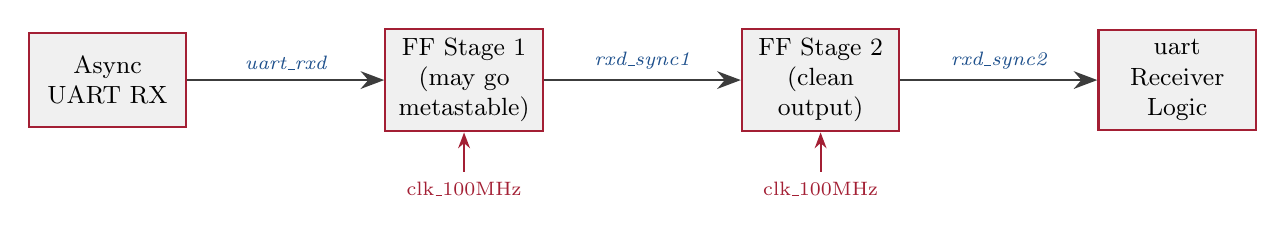
\begin{tikzpicture}[
				node distance=2cm and 2.5cm,
				block/.style={rectangle, draw=stevens, fill=lightgray, thick,
					minimum width=2cm, minimum height=1.2cm, align=center, font=\small},
				arrow/.style={-{Stealth[length=3mm]}, thick, color=darkgray},
				elabel/.style={font=\scriptsize\itshape, color=accentblue}
				]
				\node[block] (input) {Async\\UART RX};
				\node[block, right=of input] (ff1) {FF Stage 1\\(may go\\metastable)};
				\node[block, right=of ff1] (ff2) {FF Stage 2\\(clean\\output)};
				\node[block, right=of ff2] (logic) {\UART{}\\Receiver\\Logic};

				\draw[arrow] (input) -- (ff1) node[midway, above, elabel] {uart\_rxd};
				\draw[arrow] (ff1) -- (ff2) node[midway, above, elabel] {rxd\_sync1};
				\draw[arrow] (ff2) -- (logic) node[midway, above, elabel] {rxd\_sync2};

				% Clock arrows
				\draw[-{Stealth[length=2mm]}, thick, color=stevens] ($(ff1.south)+(0,-0.5)$) -- (ff1.south) node[below=0.5cm, font=\scriptsize\color{stevens}] {clk\_100MHz};
				\draw[-{Stealth[length=2mm]}, thick, color=stevens] ($(ff2.south)+(0,-0.5)$) -- (ff2.south) node[below=0.5cm, font=\scriptsize\color{stevens}] {clk\_100MHz};
			\end{tikzpicture}%
		}
		\caption{Dual-flip-flop synchronizer for the asynchronous \UART{} input. Both stages are clocked by the \FPGA{}'s 100~MHz system clock.}
		\label{fig:synchronizer}
	\end{figure}

	\begin{tcolorbox}[warning={Common Pitfalls}]
		\begin{itemize}
			\item \textbf{Skipping the synchronizer:} In simulation, the asynchronous input appears perfectly clean because the simulator resolves signals in zero time. The design will \emph{appear} to work without a synchronizer in simulation but will exhibit intermittent failures on hardware. Always include the synchronizer, even though simulation cannot demonstrate the need for it.
			\item \textbf{Synthesis attributes:} Mark the synchronizer flip-flops with the \texttt{ASYNC\_REG} attribute so that Vivado places them in the same slice, minimizing routing delay between stages:
			\begin{center}
				\texttt{attribute ASYNC\_REG : string;}\\
				\texttt{attribute ASYNC\_REG of rxd\_sync1 : signal is "TRUE";}\\
				\texttt{attribute ASYNC\_REG of rxd\_sync2 : signal is "TRUE";}
			\end{center}
			\item \textbf{Do not synchronize multi-bit buses this way.} The dual-FF synchronizer is valid only for single-bit signals. Multi-bit data crossing clock domains requires a \FIFO{} with gray-coded pointers or a handshake protocol.
		\end{itemize}
	\end{tcolorbox}

	\subsection{\UART{} Receiver Architecture}

	The \UART{} receiver samples the synchronized serial input at $16\times$ the baud rate (oversampling) to reliably detect the start bit edge and center-sample each data bit. At 115200~baud, the bit period is:

	\begin{equation}
		T_{\text{bit}} = \frac{1}{115200} \approx 8.68\;\mu\text{s}
	\end{equation}

	With a 100~MHz system clock, one bit period spans:

	\begin{equation}
		N_{\text{clk/bit}} = \frac{100 \times 10^6}{115200} \approx 868 \text{ clock cycles}
	\end{equation}

	The $16\times$ oversampling divider is:

	\begin{equation}
		N_{\text{oversample}} = \frac{N_{\text{clk/bit}}}{16} = \frac{868}{16} \approx 54 \text{ clock cycles per sample}
	\end{equation}

	\subsubsection{Receiver State Machine}

	\begin{figure}[ht!]
		\centering
		\resizebox{0.85\textwidth}{!}{%
			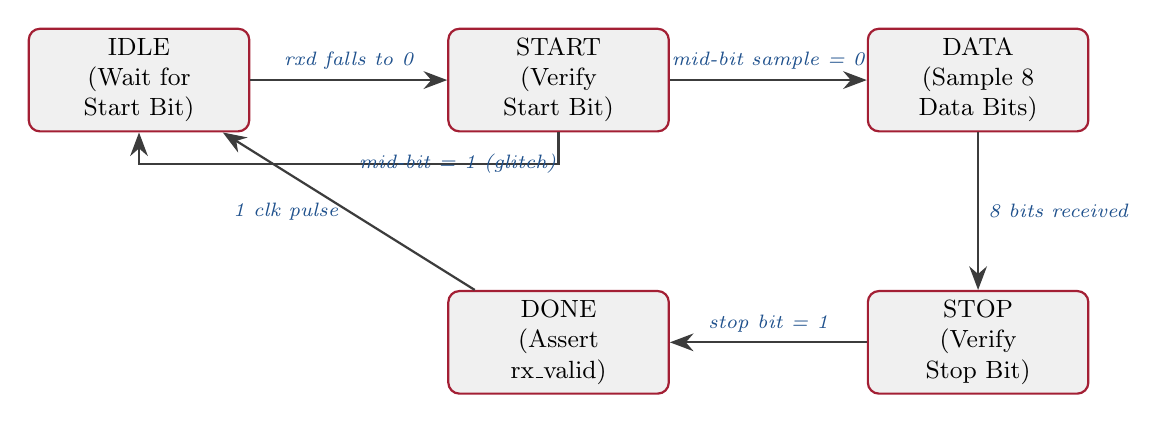
\begin{tikzpicture}[
				node distance=2cm and 2.5cm,
				state/.style={rectangle, draw=stevens, fill=lightgray, thick, rounded corners,
					minimum width=2.8cm, minimum height=1cm, align=center, font=\small},
				arrow/.style={-{Stealth[length=3mm]}, thick, color=darkgray},
				elabel/.style={font=\scriptsize\itshape, color=accentblue}
				]
				\node[state] (idle) {IDLE\\(Wait for\\Start Bit)};
				\node[state, right=of idle] (start) {START\\(Verify\\Start Bit)};
				\node[state, right=of start] (data) {DATA\\(Sample 8\\Data Bits)};
				\node[state, below=of data] (stop) {STOP\\(Verify\\Stop Bit)};
				\node[state, left=of stop] (done) {DONE\\(Assert\\rx\_valid)};

				\draw[arrow] (idle) -- (start) node[midway, above, elabel] {rxd falls to 0};
				\draw[arrow] (start) -- (data) node[midway, above, elabel] {mid-bit sample = 0};
				\draw[arrow] (start.south) -- ++(0,-0.4) -| (idle.south) node[near start, right, elabel] {mid-bit = 1 (glitch)};
				\draw[arrow] (data) -- (stop) node[midway, right, elabel] {8 bits received};
				\draw[arrow] (stop) -- (done) node[midway, above, elabel] {stop bit = 1};
				\draw[arrow] (done) -- (idle) node[midway, left, elabel] {1 clk pulse};
			\end{tikzpicture}%
		}
		\caption{\UART{} receiver state machine. The receiver waits for a falling edge (start bit), verifies at mid-bit, samples 8 data bits at their centers, checks the stop bit, and asserts a one-cycle \texttt{rx\_valid} pulse with the received byte on \texttt{rx\_data[7:0]}.}
		\label{fig:uart_fsm}
	\end{figure}

	\subsubsection{Key Design Parameters}

	\begin{table}[ht!]
		\centering
		\caption{\UART{} receiver design parameters.}
		\label{tab:uart_params}
		\renewcommand{\arraystretch}{1.3}
		\begin{tabular}{l l l}
			\toprule
			\textbf{Parameter} & \textbf{Value} & \textbf{Rationale} \\
			\midrule
			System Clock & 100~MHz & Nexys A7 on-board oscillator \\
			Baud Rate & 115200 & Matched to Module~1 receiver firmware \\
			Data Bits & 8 & Standard byte-oriented transfer \\
			Parity & None & \CRC{} provides integrity checking at frame level \\
			Stop Bits & 1 & Standard configuration \\
			Oversampling & $16\times$ & Provides $\pm 3\%$ baud rate tolerance \\
			Clocks per Sample & 54 & $\lfloor 100\text{M} / (115200 \times 16) \rfloor$ \\
			\bottomrule
		\end{tabular}
	\end{table}

	\subsubsection{Entity Interface}

	The \UART{} receiver module exposes the following port interface:

	\begin{table}[ht!]
		\centering
		\caption{\UART{} receiver entity ports.}
		\label{tab:uart_ports}
		\renewcommand{\arraystretch}{1.3}
		\begin{tabularx}{\textwidth}{l c c X}
			\toprule
			\textbf{Port} & \textbf{Direction} & \textbf{Width} & \textbf{Description} \\
			\midrule
			\texttt{clk} & in & 1 & 100~MHz system clock \\
			\texttt{rst} & in & 1 & Synchronous active-high reset \\
			\texttt{uart\_rxd} & in & 1 & Raw \UART{} serial input (asynchronous) \\
			\texttt{rx\_data} & out & 8 & Received byte (valid when \texttt{rx\_valid} = `1') \\
			\texttt{rx\_valid} & out & 1 & One-cycle pulse indicating a valid byte is available \\
			\texttt{rx\_error} & out & 1 & Framing error (stop bit not detected) \\
			\bottomrule
		\end{tabularx}
	\end{table}

	\subsection{Receive \FIFO{}}

	A small synchronous \FIFO{} decouples the byte-by-byte arrival rate of the \UART{} from the downstream packet parser, which consumes bytes in bursts (one complete frame at a time). At 115200~baud, one byte arrives every $\sim$86.8~$\mu$s (10 bit times including start and stop). A 43-byte receiver frame takes approximately 3.73~ms to arrive. The \FIFO{} must buffer at least one complete frame.

	\begin{table}[ht!]
		\centering
		\caption{Receive \FIFO{} design parameters.}
		\label{tab:fifo_params}
		\renewcommand{\arraystretch}{1.3}
		\begin{tabular}{l l l}
			\toprule
			\textbf{Parameter} & \textbf{Value} & \textbf{Rationale} \\
			\midrule
			Width & 8 bits & Byte-oriented data \\
			Depth & 64 entries & Buffers 1.4 complete frames (margin for back-pressure) \\
			Implementation & Distributed RAM & Small depth; lower latency than \BRAM{} for $\leq 64$ entries \\
			Flags & \texttt{full}, \texttt{empty}, \texttt{count[5:0]} & Parser reads when \texttt{empty} = `0'; overflow detection \\
			\bottomrule
		\end{tabular}
	\end{table}

	\begin{tcolorbox}[infobox={Design Choice: Distributed RAM vs.\ Block RAM}]
		For FIFOs of 64 entries or fewer, Vivado will infer distributed RAM (implemented in \LUT{} resources) rather than consuming a block RAM tile. This is the correct choice here: the Artix-7 100T has only 135 block RAM tiles (4,860~Kb total), and each one is a precious resource that should be reserved for larger storage needs in the feature extraction datapath (Session~7). A 64$\times$8 distributed RAM \FIFO{} consumes only 8 \LUT{}s---negligible against the 63,400 available.
	\end{tcolorbox}

	\subsection{Session 5 Integration}

	By the end of Session~5, the following modules should be implemented and individually verified in simulation:

	\begin{figure}[ht!]
		\centering
		\resizebox{0.85\textwidth}{!}{%
			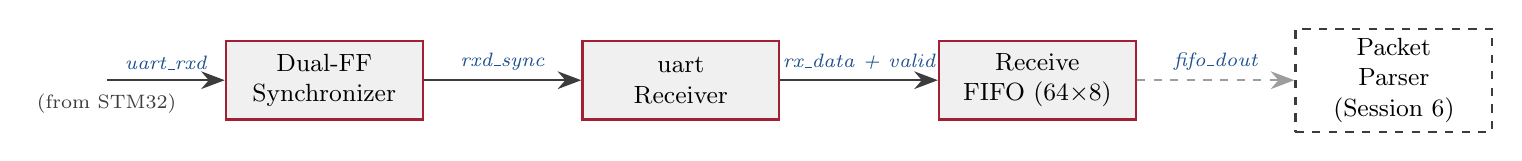
\begin{tikzpicture}[
				node distance=1.5cm and 2cm,
				block/.style={rectangle, draw=stevens, fill=lightgray, thick,
					minimum width=2.5cm, minimum height=1cm, align=center, font=\small},
				arrow/.style={-{Stealth[length=3mm]}, thick, color=darkgray},
				elabel/.style={font=\scriptsize\itshape, color=accentblue}
				]
				\node[block] (sync) {Dual-FF\\Synchronizer};
				\node[block, right=of sync] (uart) {\UART{}\\Receiver};
				\node[block, right=of uart] (fifo) {Receive\\FIFO (64$\times$8)};
				\node[block, right=of fifo, draw=darkgray, dashed, fill=white] (parser) {Packet\\Parser\\(Session 6)};

				\draw[arrow] (sync) -- (uart) node[midway, above, elabel] {rxd\_sync};
				\draw[arrow] (uart) -- (fifo) node[midway, above, elabel] {rx\_data + valid};
				\draw[arrow, dashed, color=darkgray!50] (fifo) -- (parser) node[midway, above, elabel] {fifo\_dout};

				% External input
				\draw[arrow] ($(sync.west)+(-1.5,0)$) -- (sync.west) node[midway, above, elabel] {uart\_rxd};
				\node[font=\scriptsize, color=darkgray] at ($(sync.west)+(-1.5,-0.3)$) {(from STM32)};
			\end{tikzpicture}%
		}
		\caption{Session~5 pipeline: synchronizer $\rightarrow$ \UART{} receiver $\rightarrow$ receive \FIFO{}. The dashed parser block is implemented in Session~6.}
		\label{fig:session5_pipeline}
	\end{figure}

	\begin{tcolorbox}[infobox={Exercise: \UART{} Receiver Simulation}]
		Create a \VHDL{} testbench that:
		\begin{enumerate}
			\item Generates a stimulus signal mimicking the STM32 transmitting the sequence \texttt{0x7E, 0x29, 0xA1} (the start delimiter, a frame length, and part of a timestamp) at 115200 baud. Include proper start and stop bits.
			\item Verifies that the \UART{} receiver outputs the correct bytes with the correct \texttt{rx\_valid} timing.
			\item Introduces a $\pm 2\%$ baud rate deviation in the stimulus and confirms the receiver still decodes correctly (testing the oversampling tolerance).
			\item Injects a framing error (missing stop bit) and verifies that \texttt{rx\_error} is asserted.
		\end{enumerate}
		Record waveform screenshots showing correct byte capture, \FIFO{} write, and error detection.
	\end{tcolorbox}

	\begin{tcolorbox}[deliverable={Session 5 Deliverable}]
		\textbf{\UART{} Receiver Design and Simulation Report} --- A document containing:
		\begin{enumerate}
			\item \VHDL{} source code for the synchronizer, \UART{} receiver, and receive \FIFO{} modules.
			\item Entity port descriptions and design parameter justifications.
			\item Simulation waveform captures showing correct byte reception, \FIFO{} operation, and error detection.
			\item Baud rate tolerance analysis: demonstrate correct reception at $\pm 2\%$ baud deviation and identify the failure threshold.
		\end{enumerate}
	\end{tcolorbox}

	\newpage
	% ══════════════════════════════════════════════════════════════
	\section{Session 6: Packet Parser and Frame Integrity Verification}
	\label{sec:parser}
	% ══════════════════════════════════════════════════════════════

	\subsection{Objectives}

	\begin{itemize}[leftmargin=2em]
		\item Implement a state-machine-based packet parser that detects the \texttt{0x7E} frame start delimiter and extracts the 43-byte interceptor forwarding frame structure defined in Module~1.
		\item Implement hardware \CRC{}-8 verification for the forwarding frame (transport integrity) and \CRC{}-16 verification for the embedded 32-byte radio packet (source integrity).
		\item Integrate the parser with the Session~5 \UART{} receiver and \FIFO{}.
		\item Simulate the integrated pipeline with valid and deliberately corrupted frames.
	\end{itemize}

	\subsection{Frame Structure Recap}

	The parser must handle two nested data structures. The outer structure is the interceptor-to-\FPGA{} forwarding frame defined in Module~1 (Table~6):

	\begin{table}[ht!]
		\centering
		\caption{Interceptor-to-\FPGA{} forwarding frame (43 bytes, from Module~1).}
		\label{tab:rxframe_recap}
		\renewcommand{\arraystretch}{1.3}
		\begin{tabularx}{\textwidth}{l c c X}
			\toprule
			\textbf{Field} & \textbf{Offset} & \textbf{Size} & \textbf{Description} \\
			\midrule
			Start Delimiter & 0 & 1\,B & Fixed \texttt{0x7E} \\
			Frame Length & 1 & 1\,B & Remaining frame length (excluding start delimiter and \CRC{}); always \texttt{0x29} \\
			RX Timestamp & 2 & 4\,B & Interceptor system tick (ms) \\
			\RSSI{} & 6 & 1\,B & Received signal strength (dBm, two's complement) \\
			\SNR{} & 7 & 1\,B & Signal-to-noise ratio (dB, signed) \\
			Freq.\ Error & 8 & 2\,B & Frequency error (Hz, signed 16-bit) \\
			Radio Packet & 10 & 32\,B & Complete 32-byte DATA / ACK / PAUSE packet (see inner structure) \\
			Frame \CRC{}-8 & 42 & 1\,B & \CRC{}-8 over bytes 1--41 \\
			\bottomrule
		\end{tabularx}
	\end{table}

	The inner structure is the radio packet embedded at offset~10 (Module~1, Table~4). The same 32-byte layout is used for DATA, ACK, and PAUSE; the packet type is encoded in the low two bits of the \texttt{Modulation Code} byte at offset~6 (parsed below as a separate \texttt{pkt\_type} output):

	\begin{table}[ht!]
		\centering
		\caption{Radio packet structure (32 bytes, embedded within forwarding frame; same for DATA, ACK, PAUSE).}
		\label{tab:beacon_recap}
		\renewcommand{\arraystretch}{1.3}
		\begin{tabularx}{\textwidth}{l c c X}
			\toprule
			\textbf{Field} & \textbf{Offset} & \textbf{Size} & \textbf{Description} \\
			\midrule
			Preamble Sync & 0 & 2\,B & \texttt{0xAE5A} (frame detection) \\
			Beacon ID & 2 & 1\,B & Sender ID (Target~A=\texttt{0x01}, Target~B=\texttt{0x02}, Threat=\texttt{0xFF}) \\
			Sequence Number & 3 & 2\,B & Packet loss detection counter; for ACK echoes the acknowledged DATA's sequence \\
			TX Power & 5 & 1\,B & Transmit power (dBm) \\
			Modulation Code & 6 & 1\,B & Packed: bits[7:2] = mod kind (\texttt{0x01}=LoRa, \texttt{0x02}=\FSK{}, \texttt{0x03}=\OOK{}, $\ll$2); bits[1:0] = pkt type (\texttt{00}=DATA, \texttt{01}=ACK, \texttt{10}=PAUSE) \\
			Spreading Factor & 7 & 1\,B & SF7--SF12; 0x00 if non-LoRa \\
			Bandwidth Code & 8 & 1\,B & 0x00=125kHz, 0x01=250kHz \\
			Timestamp & 9 & 4\,B & Sender-side system tick (ms) \\
			Payload (DATA/ACK) or PAUSE args & 13 & 17\,B & DATA/ACK: pseudo-random or user data. PAUSE: byte~0 = target ID, byte~1 = hold-off in 100\,ms units, bytes 2--16 = \texttt{0xAA} fill \\
			\CRC{}-16 & 30 & 2\,B & \CRC{}-16/CCITT-FALSE over bytes 0--29 \\
			\bottomrule
		\end{tabularx}
	\end{table}

	\subsection{Packet Parser State Machine}

	The parser reads bytes sequentially from the receive \FIFO{} and walks through the frame structure field by field. A byte counter tracks the current position within the frame, and dedicated registers capture each field as it arrives.

	\begin{figure}[ht!]
		\centering
		\resizebox{\textwidth}{!}{%
			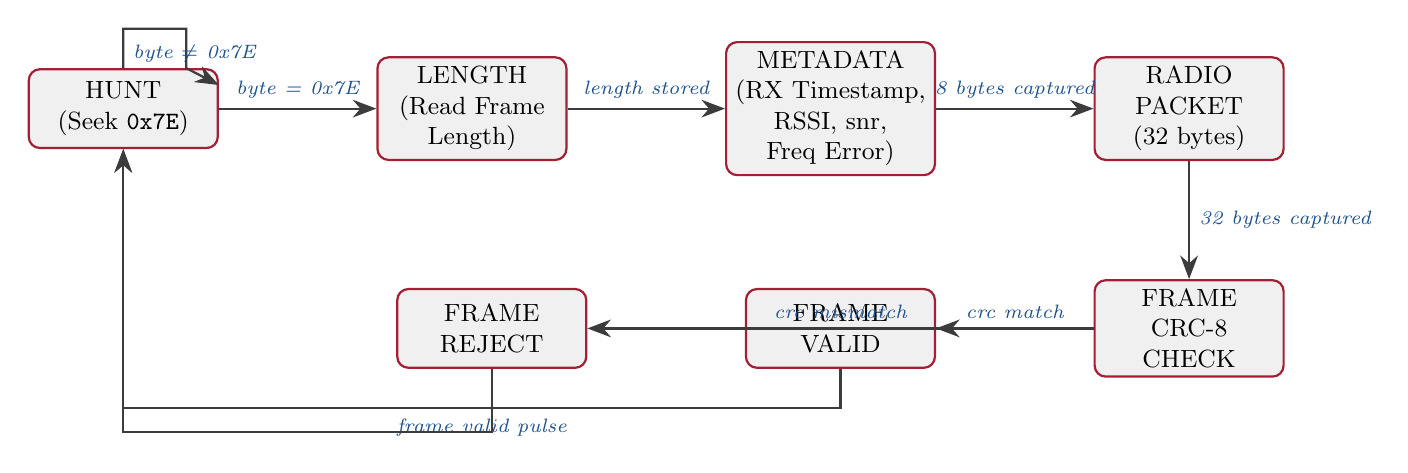
\begin{tikzpicture}[
				node distance=1.5cm and 2cm,
				state/.style={rectangle, draw=stevens, fill=lightgray, thick, rounded corners,
					minimum width=2.4cm, minimum height=1cm, align=center, font=\small},
				arrow/.style={-{Stealth[length=3mm]}, thick, color=darkgray},
				elabel/.style={font=\scriptsize\itshape, color=accentblue}
				]
				\node[state] (hunt) {HUNT\\(Seek \texttt{0x7E})};
				\node[state, right=of hunt] (len) {LENGTH\\(Read Frame\\Length)};
				\node[state, right=of len] (meta) {METADATA\\(RX Timestamp,\\RSSI, \SNR{},\\Freq Error)};
				\node[state, right=of meta] (payload) {RADIO\\PACKET\\(32 bytes)};
				\node[state, below=of payload] (crc) {FRAME\\CRC-8\\CHECK};
				\node[state, left=of crc] (valid) {FRAME\\VALID};
				\node[state, left=of valid] (reject) {FRAME\\REJECT};

				\draw[arrow] (hunt) -- (len) node[midway, above, elabel] {byte = 0x7E};
				\draw[arrow] (len) -- (meta) node[midway, above, elabel] {length stored};
				\draw[arrow] (meta) -- (payload) node[midway, above, elabel] {8 bytes captured};
				\draw[arrow] (payload) -- (crc) node[midway, right, elabel] {32 bytes captured};
				\draw[arrow] (crc) -- (valid) node[midway, above, elabel] {\CRC{} match};
				\draw[arrow] (crc) -- (reject) node[midway, above, elabel] {\CRC{} mismatch};
				\draw[arrow] (valid.south) -- ++(0,-0.5) -| (hunt.south) node[near start, below, elabel] {frame\_valid pulse};
				\draw[arrow] (reject.south) -- ++(0,-0.8) -| (hunt.south);

				% Self-loop on hunt
				\draw[arrow] (hunt.north) -- ++(0,0.5) -| ($(hunt.north)+(0.8,0)$) -- ($(hunt.east)+(0,0.3)$) node[near start, above, elabel] {byte $\neq$ 0x7E};
			\end{tikzpicture}%
		}
		\caption{Packet parser state machine. The HUNT state discards bytes until the start delimiter is found. The parser then progresses through fixed-length fields sequentially, culminating in \CRC{} verification. On \CRC{} failure, the parser returns to HUNT without asserting \texttt{frame\_valid}.}
		\label{fig:parser_fsm}
	\end{figure}

	\subsubsection{Parser Entity Interface}

	\begin{table}[ht!]
		\centering
		\caption{Packet parser entity ports.}
		\label{tab:parser_ports}
		\renewcommand{\arraystretch}{1.3}
		\begin{tabularx}{\textwidth}{l c c X}
			\toprule
			\textbf{Port} & \textbf{Dir} & \textbf{Width} & \textbf{Description} \\
			\midrule
			\texttt{clk} & in & 1 & 100~MHz system clock \\
			\texttt{rst} & in & 1 & Synchronous active-high reset \\
			\texttt{fifo\_data} & in & 8 & Byte from receive \FIFO{} \\
			\texttt{fifo\_empty} & in & 1 & \FIFO{} empty flag \\
			\texttt{fifo\_rd} & out & 1 & \FIFO{} read enable (parser requests next byte) \\
			\texttt{frame\_valid} & out & 1 & One-cycle pulse: complete frame passed \CRC{} \\
			\texttt{frame\_reject} & out & 1 & One-cycle pulse: frame failed \CRC{} \\
			\texttt{rx\_timestamp} & out & 32 & Receiver timestamp field \\
			\texttt{rssi} & out & 8 & \RSSI{} field \\
			\texttt{snr} & out & 8 & \SNR{} field \\
			\texttt{freq\_error} & out & 16 & Frequency error field \\
			\texttt{beacon\_id} & out & 8 & Beacon ID from embedded payload \\
			\texttt{seq\_num} & out & 16 & Beacon sequence number \\
			\texttt{tx\_power} & out & 8 & Sender TX power (dBm) \\
			\texttt{mod\_kind} & out & 6 & Upper 6 bits of \texttt{Modulation Code}: modulation kind (LoRa / FSK / OOK encoded $\ll$2) \\
			\texttt{pkt\_type} & out & 2 & Low 2 bits of \texttt{Modulation Code}: \texttt{00}=DATA, \texttt{01}=ACK, \texttt{10}=PAUSE \\
			\texttt{spread\_factor} & out & 8 & Spreading factor \\
			\texttt{bw\_code} & out & 8 & Bandwidth code \\
			\texttt{sender\_timestamp} & out & 32 & Sender-side timestamp \\
			\texttt{pause\_target\_id} & out & 8 & Valid only when \texttt{pkt\_type} = \texttt{10}: target Beacon~ID being paused (radio payload byte~0) \\
			\texttt{pause\_duration\_units} & out & 8 & Valid only when \texttt{pkt\_type} = \texttt{10}: hold-off in 100\,ms units (radio payload byte~1) \\
			\texttt{packet\_crc\_ok} & out & 1 & Inner \CRC{}-16 verification result \\
			\bottomrule
		\end{tabularx}
	\end{table}

	\subsection{Hardware \CRC{} Implementation}

	The pipeline performs two levels of \CRC{} verification. The \CRC{}-8 check validates transport integrity (did the bytes survive the \UART{} link without corruption?), while the \CRC{}-16 check validates source integrity (did the originating station construct the packet correctly?). Both checks execute in hardware as the bytes stream through the parser, adding zero latency to the overall frame processing time.

	\subsubsection{\CRC{}-8 (Frame Transport Integrity)}

	The receiver frame uses \CRC{}-8 with the polynomial:

	\begin{equation}
		G(x) = x^8 + x^2 + x + 1 \quad \text{(0x07, \CRC{}-8/ITU)}
		\label{eq:crc8}
	\end{equation}

	The \CRC{} is computed over bytes 1--41 of the frame (everything between the start delimiter and the \CRC{} byte itself). The hardware implementation uses a byte-wide combinational \CRC{} step function: each time a new byte arrives from the parser, the current \CRC{} register is updated in a single clock cycle.

	The byte-wide \CRC{}-8 update can be expressed as a set of XOR equations derived from the polynomial. For an 8-bit input byte $D[7{:}0]$ and current \CRC{} state $C[7{:}0]$, the next \CRC{} state $C'[7{:}0]$ is a purely combinational function:

	\begin{equation}
		C'[i] = f_i(C[7{:}0], D[7{:}0]) \quad \text{for } i = 0, 1, \ldots, 7
		\label{eq:crc8_update}
	\end{equation}

	where each $f_i$ is an XOR tree that can be generated automatically by tools or derived from the polynomial long division.

	\begin{tcolorbox}[infobox={Implementation Strategy: \CRC{} XOR Equations}]
		Rather than implementing \CRC{} bit-by-bit (which would require 8 clock cycles per byte), use a pre-computed byte-wide XOR network. The open-source tool \texttt{pycrc} or the online OutputLogic \CRC{} Generator can produce the \VHDL{} combinational equations for any polynomial and data width. For \CRC{}-8/0x07 with 8-bit data input, this yields 8 XOR equations, each involving a subset of the 16 input bits ($C[7{:}0]$ and $D[7{:}0]$). The entire update computes in a single combinational step.
	\end{tcolorbox}

	\subsubsection{\CRC{}-16 (Radio Packet Integrity)}

	The radio packet uses \CRC{}-16-CCITT:

	\begin{equation}
		G(x) = x^{16} + x^{12} + x^5 + 1 \quad \text{(0x1021)}
		\label{eq:crc16}
	\end{equation}

	This \CRC{} is computed over bytes 0--29 of the radio packet (the first 30 bytes within the 32-byte packet embedded at frame offset~10). The same byte-wide combinational approach applies: a 16-bit \CRC{} register is updated once per byte as the parser streams through the radio packet region.

	\subsubsection{\CRC{} Verification Timing}

	\begin{figure}[ht!]
		\centering
		\resizebox{\textwidth}{!}{%
			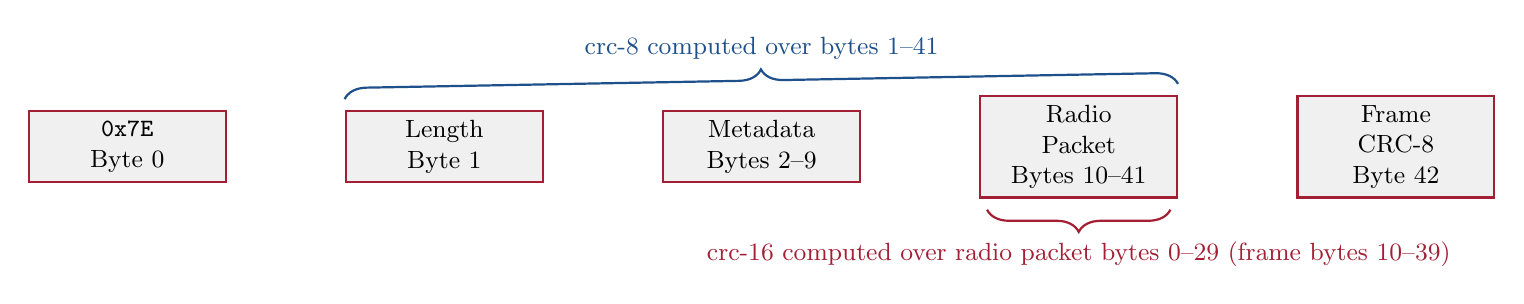
\begin{tikzpicture}[
				node distance=1.2cm and 1.5cm,
				block/.style={rectangle, draw=stevens, fill=lightgray, thick,
					minimum width=2.5cm, minimum height=0.9cm, align=center, font=\small},
				crc/.style={rectangle, draw=accentblue, fill=blue!5, thick,
					minimum width=2.5cm, minimum height=0.9cm, align=center, font=\small},
				arrow/.style={-{Stealth[length=3mm]}, thick, color=darkgray},
				elabel/.style={font=\scriptsize\itshape, color=accentblue}
				]
				% Frame bytes
				\node[block] (delim) {\texttt{0x7E}\\Byte 0};
				\node[block, right=of delim] (len) {Length\\Byte 1};
				\node[block, right=of len] (meta) {Metadata\\Bytes 2--9};
				\node[block, right=of meta] (bpay) {Radio\\Packet\\Bytes 10--41};
				\node[block, right=of bpay] (fcrc) {Frame\\CRC-8\\Byte 42};

				% \CRC{}-8 span
				\draw[decorate, decoration={brace, amplitude=8pt, raise=4pt}, thick, color=accentblue]
				(len.north west) -- (bpay.north east)
				node[midway, above=12pt, font=\small\color{accentblue}] {\CRC{}-8 computed over bytes 1--41};

				% \CRC{}-16 span
				\draw[decorate, decoration={brace, amplitude=8pt, raise=4pt, mirror}, thick, color=stevens]
				($(bpay.south west)+(0.1,0)$) -- ($(bpay.south east)+(-0.1,0)$)
				node[midway, below=12pt, font=\small\color{stevens}] {\CRC{}-16 computed over radio packet bytes 0--29 (frame bytes 10--39)};
			\end{tikzpicture}%
		}
		\caption{\CRC{} coverage within the forwarding frame. \CRC{}-8 covers the entire frame body. \CRC{}-16 covers the radio packet (DATA / ACK / PAUSE) independently. Both are computed concurrently as bytes stream through the parser.}
		\label{fig:crc_coverage}
	\end{figure}

	\begin{tcolorbox}[warning={Common Pitfalls}]
		\begin{itemize}
			\item \textbf{\CRC{} initialization:} \CRC{}-8/ITU initializes to \texttt{0x00}; \CRC{}-16-CCITT initializes to \texttt{0xFFFF}. Incorrect initialization will produce a valid-looking but wrong \CRC{} for every frame, causing 100\% rejection.
			\item \textbf{Byte ordering:} The \CRC{}-16 check bytes in the radio packet are transmitted MSB-first. Ensure the comparison logic accounts for the byte order of the received \CRC{} field versus the computed residual.
			\item \textbf{Running \CRC{} during non-covered bytes:} The \CRC{}-8 engine must \emph{not} include byte~0 (the start delimiter) in its computation. The \CRC{}-16 engine must only process the 30 radio packet data bytes (frame bytes 10--39), not the 2-byte \CRC{}-16 field itself (bytes 40--41). Use the parser's byte counter to gate the \CRC{} update enable signals.
		\end{itemize}
	\end{tcolorbox}

	\subsection{Integrated Parser Simulation}

	\begin{tcolorbox}[infobox={Exercise: Parser Verification with Module~1 Data}]
		Create a simulation testbench that:
		\begin{enumerate}
			\item Feeds a sequence of valid 43-byte frames (recorded or hand-constructed from Module~1 packet format) through the \UART{} receiver and into the parser. Verify that all parsed fields match expected values and \texttt{frame\_valid} is asserted for each frame.
			\item Inserts a single corrupted byte (bit flip) in the metadata region of one frame. Verify that \CRC{}-8 fails and \texttt{frame\_reject} is asserted while subsequent valid frames still parse correctly.
			\item Inserts a corrupted byte within the radio packet region. Verify that the frame-level \CRC{}-8 still fails (the corruption propagates through both \CRC{} engines) and the packet-level \CRC{}-16 also reports failure via \texttt{packet\_crc\_ok} = `0'.
			\item Sends a stream of bytes with \emph{no} \texttt{0x7E} delimiter for 100 bytes, then sends a valid frame. Verify that the parser remains in HUNT state during the garbage bytes and correctly synchronizes when the valid frame arrives.
			\item Tests back-to-back frames with zero inter-frame gap. Verify the parser immediately re-enters HUNT and captures the second frame.
		\end{enumerate}
	\end{tcolorbox}

	\begin{tcolorbox}[deliverable={Session 6 Deliverable}]
		\textbf{Packet Parser and \CRC{} Verification Report} --- A document containing:
		\begin{enumerate}
			\item \VHDL{} source code for the packet parser state machine, \CRC{}-8 module, and \CRC{}-16 module.
			\item State machine diagram with transition conditions and output assignments.
			\item Simulation waveform captures demonstrating: valid frame parsing, \CRC{}-8 rejection, \CRC{}-16 rejection, synchronization recovery, and back-to-back frame handling.
			\item A table comparing expected vs.\ actual parsed field values for at least 5 distinct test frames.
		\end{enumerate}
	\end{tcolorbox}

	\newpage
	% ══════════════════════════════════════════════════════════════
	\section{Session 7: Feature Extraction Datapath}
	\label{sec:feature}
	% ══════════════════════════════════════════════════════════════

	\subsection{Objectives}

	\begin{itemize}[leftmargin=2em]
		\item Define a fixed-format feature vector that captures the signal characteristics needed by the \ML{} classification pipeline in Module~4.
		\item Implement a feature extraction module that populates the feature vector from parsed packet fields.
		\item Design a dual-port block RAM storage structure for accumulating feature vectors from multiple stations (Target~A, Target~B, and the Threat).
		\item Implement station prioritization logic based on received signal quality metrics.
		\item Provide a host-readable output interface for exporting feature vectors to the \ML{} pipeline.
	\end{itemize}

	\subsection{Feature Vector Design}

	The feature vector is the data product of the \FPGA{} pipeline---the structured representation of each intercepted DATA, ACK, or PAUSE transmission that will serve as input to the machine learning classifiers in Module~4. Its design is a cross-domain decision: the \FPGA{} designer must include enough information for the \ML{} engineer to build accurate classifiers (including ground-truth labels for SF, modulation kind, emitter ID, and packet type), but the vector must remain compact enough to store and export efficiently within the \FPGA{}'s resource budget.

	\begin{tcolorbox}[infobox={Design Principle: Features as Cross-Domain Interface}]
		The feature vector is the primary data contract between the \FPGA{} pipeline (Module~2) and the \ML{} classification pipeline (Module~4). Decisions made here---which fields to include, their precision, and their ordering---directly constrain the preprocessing and model architecture decisions students make two modules later. This is a concrete example of the cross-domain interface reasoning the framework is designed to teach: an \FPGA{} design choice shapes an \ML{} workflow.
	\end{tcolorbox}

	\subsubsection{Feature Vector Format}

	\begin{table}[ht!]
		\centering
		\caption{Feature vector format (32 bytes per intercepted-packet observation).}
		\label{tab:feature_vector}
		\renewcommand{\arraystretch}{1.3}
		\begin{tabularx}{\textwidth}{l c c X}
			\toprule
			\textbf{Field} & \textbf{Offset} & \textbf{Size} & \textbf{Description / \ML{} Relevance} \\
			\midrule
			Beacon ID & 0 & 1\,B & Class label for emitter identification tasks. \\
			Modulation Kind & 1 & 1\,B & Ground-truth label for modulation classification. Holds the upper 6 bits of the radio packet's \texttt{Modulation Code} byte (right-shifted by 2 so the value is the canonical \texttt{0x01}=LoRa / \texttt{0x02}=FSK / \texttt{0x03}=OOK), with the low 2 bits cleared. \\
			Spreading Factor & 2 & 1\,B & Ground-truth label for SF detection tasks. \\
			\texttt{pkt\_type} & 3 & 1\,B & Ground-truth label for packet-type classification: \texttt{0x00}=DATA, \texttt{0x01}=ACK, \texttt{0x02}=PAUSE. Extracted from the low 2 bits of the radio packet's \texttt{Modulation Code} byte. \\
			TX Power & 4 & 1\,B & Transmitted power (enables path loss estimation). \\
			\RSSI{} & 5 & 1\,B & Primary signal strength feature (signed). \\
			\SNR{} & 6 & 1\,B & Signal quality feature (signed). \\
			Freq.\ Error & 7 & 2\,B & Carrier offset feature (signed, Hz). \\
			RX Timestamp & 9 & 4\,B & Absolute reception time at the interceptor. \\
			Sender Timestamp & 13 & 4\,B & Transmission time (enables latency calculation). \\
			Sequence Number & 17 & 2\,B & Packet loss and ordering feature. \\
			Payload \CRC{} Status & 19 & 1\,B & 0x01 = pass, 0x00 = fail (data quality indicator). \\
			Inter-Arrival Time & 20 & 4\,B & Time since last packet from this Beacon~ID (computed). \\
			\RSSI{} Delta & 24 & 2\,B & Change in \RSSI{} from previous observation (computed, signed). \\
			Observation Count & 26 & 2\,B & Running count of observations from this Beacon~ID. \\
			\texttt{target\_id\_if\_pause} & 28 & 1\,B & Only meaningful when \texttt{pkt\_type} = PAUSE: target Beacon~ID being paused (radio payload byte~0); zero otherwise. \\
			\texttt{pause\_duration\_units} & 29 & 1\,B & Only meaningful when \texttt{pkt\_type} = PAUSE: hold-off in 100\,ms units (radio payload byte~1); zero otherwise. \\
			Reserved & 30 & 2\,B & Padding for 32-byte alignment; available for future features. \\
			\bottomrule
		\end{tabularx}
	\end{table}

	\subsubsection{Computed Features}

	Most feature-vector fields are direct copies or simple bit-field extractions from the parsed radio packet --- including the \texttt{pkt\_type} field at offset~3 (low 2 bits of \texttt{Modulation Code}), the Modulation Kind field at offset~1 (upper 6 bits of \texttt{Modulation Code} right-shifted by 2), and the \texttt{target\_id\_if\_pause} / \texttt{pause\_duration\_units} fields at offsets~28--29 (radio payload bytes~0--1, valid only when \texttt{pkt\_type} = PAUSE). Three fields, however, are not directly extracted from the packet but are computed by the \FPGA{} logic from the current and previous observations:

	\begin{itemize}[leftmargin=2em]
		\item \textbf{Inter-Arrival Time:} The difference between the current RX timestamp and the RX timestamp of the last valid packet from the same Beacon~ID. This feature captures transmission scheduling regularity, which differs between scheduling modes (TDMA vs.\ ALOHA), between packet types (1-second DATA cadence vs.\ event-driven ACK vs.\ 100~ms PAUSE bursts), and is a useful discriminator for the \ML{} pipeline.

		\begin{equation}
			\Delta t_{\text{IAT}}^{(k)} = T_{\text{rx,current}}^{(k)} - T_{\text{rx,previous}}^{(k)}
			\label{eq:iat}
		\end{equation}

		where $k$ is the Beacon ID.

		\item \textbf{\RSSI{} Delta:} The signed difference between the current \RSSI{} and the \RSSI{} of the previous observation from the same station. Large \RSSI{} fluctuations may indicate multipath fading, obstruction, or power control changes---all of which are relevant to anomaly detection tasks.

		\begin{equation}
			\Delta \text{\RSSI{}}^{(k)} = \text{\RSSI{}}_{\text{current}}^{(k)} - \text{\RSSI{}}_{\text{previous}}^{(k)}
			\label{eq:rssi_delta}
		\end{equation}

		\item \textbf{Observation Count:} A running counter of valid frames received from each Beacon~ID since reset. This provides a measure of link reliability and can serve as a weight or confidence indicator in the \ML{} pipeline.
	\end{itemize}

	\begin{tcolorbox}[warning={Common Pitfalls}]
		\begin{itemize}
			\item \textbf{First-observation edge case:} When a station is seen for the first time (observation count = 1), there is no previous timestamp or \RSSI{}. Set Inter-Arrival Time to \texttt{0xFFFFFFFF} (sentinel) and \RSSI{} Delta to \texttt{0x0000}. The \ML{} preprocessing code in Module~4 must be aware of these sentinel values.
			\item \textbf{Timestamp rollover:} The STM32 system tick is a 32-bit millisecond counter that rolls over after $\sim$49.7 days. For benchtop sessions this is not a concern, but the subtraction logic should use unsigned arithmetic to handle rollover correctly in principle.
			\item \textbf{Signed vs.\ unsigned:} \RSSI{} (two's complement) and Freq.\ Error (signed 16-bit) are signed quantities. Ensure the \VHDL{} arithmetic uses \texttt{signed} types from \texttt{ieee.numeric\_std} for delta computations.
		\end{itemize}
	\end{tcolorbox}

	\subsection{Per-Station State Registers}

	To compute the derived features, the \FPGA{} must maintain per-station state. A small register file indexed by Beacon~ID stores the previous observation's timestamp, \RSSI{}, and the running observation count. The same RAM holds entries for both cooperative targets (Target~A=\texttt{0x01}, Target~B=\texttt{0x02}) and the interceptor (Threat=\texttt{0xFF}); state for the latter is populated only when the Threat's own PAUSE transmissions are caught off-air, which is unusual due to the interceptor's half-duplex shadow but is observable in some bench geometries.

	\begin{table}[ht!]
		\centering
		\caption{Per-station state storage (7 bytes per Beacon~ID).}
		\label{tab:beacon_state}
		\renewcommand{\arraystretch}{1.3}
		\begin{tabularx}{\textwidth}{l c X}
			\toprule
			\textbf{Field} & \textbf{Size} & \textbf{Description} \\
			\midrule
			Previous RX Timestamp & 4\,B & Last valid reception time for this Beacon~ID \\
			Previous \RSSI{} & 1\,B & Last \RSSI{} value for this Beacon~ID \\
			Observation Count & 2\,B & Running count of valid observations \\
			\bottomrule
		\end{tabularx}
	\end{table}

	With Beacon~IDs ranging from \texttt{0x01} to \texttt{0xFF} (255 possible senders), the state register file requires $255 \times 7 = 1{,}785$ bytes. This fits comfortably in a single 2~KB block RAM tile (one 18~Kb \BRAM{} configured as $256 \times 8$, or a pair of them for wider access).

	\begin{tcolorbox}[infobox={Design Choice: Register File vs.\ Lookup Table}]
		For the expected benchtop scenario of 2--3 active stations (Target~A, Target~B, and occasionally the Threat), a simple array of registers would suffice and avoid the \BRAM{} overhead. However, implementing the state as an addressable RAM indexed by Beacon~ID scales cleanly to the full 255-sender address space without modification. This is a deliberate pedagogical choice: students learn to design for the general case using parameterizable, memory-mapped structures rather than hard-coding for a specific station count. The \BRAM{} cost (1 tile out of 135) is minimal.
	\end{tcolorbox}

	\subsection{Feature Storage: Dual-Port Block RAM}

	Completed feature vectors are written to a dual-port block RAM that serves as the handoff buffer between the \FPGA{} pipeline and the host-side \ML{} data collection. Port~A is the \FPGA{} write port (driven by the feature extraction logic); Port~B is the read port (driven by the host interface for data export).

	\begin{table}[ht!]
		\centering
		\caption{Feature storage \BRAM{} configuration.}
		\label{tab:feature_bram}
		\renewcommand{\arraystretch}{1.3}
		\begin{tabular}{l l l}
			\toprule
			\textbf{Parameter} & \textbf{Value} & \textbf{Rationale} \\
			\midrule
			Width & 256 bits (32 bytes) & One feature vector per address \\
			Depth & 256 entries & One slot per possible Beacon~ID \\
			Total Size & 8~KB & Fits in 4$\times$ 18~Kb \BRAM{} tiles (or 2$\times$ 36~Kb) \\
			Port A & Write (\FPGA{} pipeline) & Synchronous write on \texttt{frame\_valid} \\
			Port B & Read (host interface) & Asynchronous read for data export via \UART{} \\
			\bottomrule
		\end{tabular}
	\end{table}

	\subsubsection{Write Logic}

	When the parser asserts \texttt{frame\_valid}, the feature extraction module:
	\begin{enumerate}[leftmargin=2em]
		\item Reads the per-station state for the incoming Beacon~ID from the state RAM.
		\item Computes the three derived features (Inter-Arrival Time, \RSSI{} Delta, Observation Count).
		\item Extracts the bit-field-packed fields from the parser outputs: \texttt{pkt\_type} from the low 2 bits of \texttt{mod\_code}, Modulation Kind from the upper 6 bits.
		\item Copies the PAUSE-only fields from the parser's \texttt{pause\_target\_id} and \texttt{pause\_duration\_units} outputs into feature-vector offsets~28--29 (zeroed when \texttt{pkt\_type} $\ne$ PAUSE).
		\item Assembles the 32-byte feature vector.
		\item Writes the feature vector to the feature \BRAM{} at address = Beacon~ID.
		\item Updates the per-station state RAM with the current timestamp, \RSSI{}, and incremented count.
	\end{enumerate}

	This sequence completes in a small fixed number of clock cycles (state read latency + computation + write = $\sim$4--6 cycles at 100~MHz), which is negligible compared to the $\sim$3.73~ms frame arrival interval at 115200 baud.

	\subsubsection{Read / Export Interface}

	For Module~2, the export interface is a simple \UART{} transmitter that sends feature vectors to the host PC on demand (triggered by a pushbutton or a host-side \UART{} command). The host-side Python script stores the received feature vectors as CSV or binary records for use in Module~4. The full export protocol is finalized during Module~3 integration, but the \BRAM{} read port and a minimal \UART{} TX module should be implemented now to enable early testing.

	\subsection{Station Prioritization Logic}

	As a stretch goal for advanced students, implement a simple prioritization scheme that ranks active stations by signal quality. The priority score for each Beacon~ID can be computed as:

	\begin{equation}
		P^{(k)} = \alpha \cdot \text{\RSSI{}}^{(k)} + \beta \cdot \text{\SNR{}}^{(k)} - \gamma \cdot |\Delta \text{\RSSI{}}^{(k)}|
		\label{eq:priority}
	\end{equation}

	where $\alpha$, $\beta$, and $\gamma$ are configurable 8-bit weight registers. The station with the highest priority score is indicated on the Nexys A7 seven-segment display, providing a real-time visual indicator of the ``best'' signal source. This is also conceptually the same selection rule the Module~1 Threat firmware uses to pick its PAUSE target, evaluated here in hardware rather than firmware. This exercise introduces students to parameterized hardware arithmetic and prepares them for the concept of hardware-accelerated inference in Module~4.

	\subsection{Session 7 Pipeline Architecture}

	\begin{figure}[ht!]
		\centering
		\resizebox{\textwidth}{!}{%
			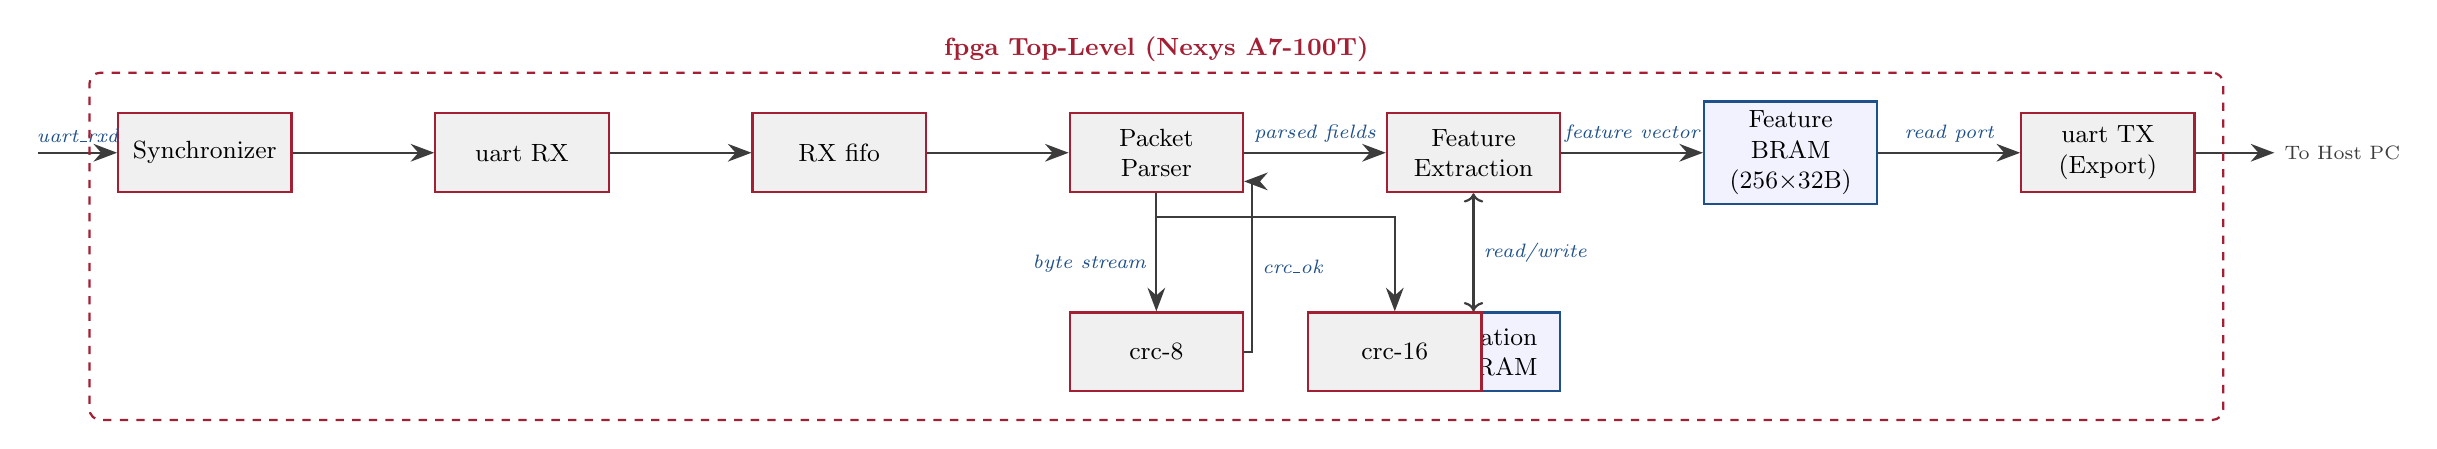
\begin{tikzpicture}[
				node distance=1.2cm and 1.8cm,
				block/.style={rectangle, draw=stevens, fill=lightgray, thick,
					minimum width=2.2cm, minimum height=1cm, align=center, font=\small},
				mem/.style={rectangle, draw=accentblue, fill=blue!5, thick,
					minimum width=2.2cm, minimum height=1cm, align=center, font=\small},
				arrow/.style={-{Stealth[length=3mm]}, thick, color=darkgray},
				elabel/.style={font=\scriptsize\itshape, color=accentblue}
				]
				% Pipeline
				\node[block] (sync) {Synchronizer};
				\node[block, right=of sync] (uart) {\UART{} RX};
				\node[block, right=of uart] (fifo) {RX \FIFO{}};
				\node[block, right=of fifo] (parser) {Packet\\Parser};
				\node[block, right=of parser] (feat) {Feature\\Extraction};
				\node[mem, right=of feat] (bram) {Feature\\BRAM\\(256$\times$32B)};
				\node[block, right=of bram] (export) {\UART{} TX\\(Export)};

				% State RAM
				\node[mem, below=1.5cm of feat] (state) {Per-Station\\State RAM};

				% \CRC{} modules
				\node[block, below=1.5cm of parser] (crc8) {\CRC{}-8};
				\node[block, right=0.8cm of crc8] (crc16) {\CRC{}-16};

				% Arrows
				\draw[arrow] ($(sync.west)+(-1,0)$) -- (sync.west) node[midway, above, elabel] {uart\_rxd};
				\draw[arrow] (sync) -- (uart);
				\draw[arrow] (uart) -- (fifo);
				\draw[arrow] (fifo) -- (parser);
				\draw[arrow] (parser) -- (feat) node[midway, above, elabel] {parsed fields};
				\draw[arrow] (feat) -- (bram) node[midway, above, elabel] {feature vector};
				\draw[arrow] (bram) -- (export) node[midway, above, elabel] {read port};
				\draw[arrow] (export.east) -- ++(1,0) node[right, font=\scriptsize] {To Host PC};

				% \CRC{} connections
				\draw[arrow] (parser.south) -- ++(0,-0.3) -| (crc8.north) node[near end, left, elabel] {byte stream};
				\draw[arrow] (parser.south) -- ++(0,-0.3) -| (crc16.north);
				\draw[arrow] (crc8.east) -- ++(0.1,0) |- ($(parser.south east)+(0,0.15)$) node[near start, right, elabel] {crc\_ok};

				% State RAM connections
				\draw[arrow, <->] (feat.south) -- (state.north) node[midway, right, elabel] {read/write};

				% Grouping
				\node[draw=stevens, dashed, thick, rounded corners,
				fit=(sync)(uart)(fifo)(parser)(feat)(bram)(export)(state)(crc8)(crc16),
				inner sep=10pt,
				label={[font=\small\bfseries\color{stevens}]above:\FPGA{} Top-Level (Nexys A7-100T)}] {};
			\end{tikzpicture}%
		}
		\caption{Complete Module~2 \FPGA{} pipeline architecture. Solid blocks are implemented across Sessions~5--7. The \UART{} TX export module enables early data extraction for \ML{} pipeline prototyping.}
		\label{fig:full_pipeline}
	\end{figure}

	\begin{tcolorbox}[infobox={Exercise: Feature Vector Verification}]
		Using the cooperative-target ping-pong (Target~A initiator, Target~B responder) plus interleaved PAUSE traffic, all from Module~1:
		\begin{enumerate}
			\item Run the full \FPGA{} pipeline in simulation for 30 simulated seconds of intercepted traffic (approximately 30 DATA packets from Target~A, 30 ACKs from Target~B at 1-second ping-pong cadence, plus 50 PAUSE packets from a 5-second simulated button-hold at 100\,ms cadence).
			\item Export the feature \BRAM{} contents and verify:
			\begin{itemize}
				\item Beacon~IDs \texttt{0x01} (Target~A), \texttt{0x02} (Target~B), and \texttt{0xFF} (Threat) each have entries in the \BRAM{}.
				\item The \texttt{pkt\_type} field at offset~3 differs across the three rows: Target~A's row is dominated by DATA (\texttt{0x00}), Target~B's by ACK (\texttt{0x01}), and the Threat's (if captured) by PAUSE (\texttt{0x02}).
				\item For the Threat's row, \texttt{target\_id\_if\_pause} (offset~28) is non-zero and \texttt{pause\_duration\_units} (offset~29) is \texttt{0x05} (500\,ms).
				\item \RSSI{} values differ between Target~A and Target~B (reflecting their distance / TX-power difference from Module~1).
				\item Observation counts increment correctly for each station.
				\item Inter-arrival times are approximately 1000~ms for Target~A (DATA cadence) and similar for Target~B (each ACK follows a DATA).
				\item \RSSI{} Delta values are near zero for fixed-position, fixed-power stations.
			\end{itemize}
			\item Introduce a 5~dB TX power reduction on Target~B midway through the simulation. Verify that Target~B's \RSSI{} Delta becomes negative and the feature vector captures the transition.
		\end{enumerate}
	\end{tcolorbox}

	\begin{tcolorbox}[deliverable={Session 7 Deliverable}]
		\textbf{Feature Extraction Datapath Design Document} --- A document containing:
		\begin{enumerate}
			\item Feature vector format specification with field descriptions, sizes, and \ML{} relevance.
			\item \VHDL{} source code for the feature extraction module, per-station state RAM, and feature \BRAM{}.
			\item Block diagram of the complete pipeline from \UART{} input to feature \BRAM{} output.
			\item Simulation results demonstrating correct feature computation for multi-station scenarios (cooperative-target ping-pong with interleaved PAUSE bursts), including computed features (inter-arrival time, \RSSI{} delta, observation count) and the bit-field-extracted \texttt{pkt\_type} column.
			\item Resource estimate: anticipated \LUT{}, FF, and \BRAM{} usage for the current design.
		\end{enumerate}
	\end{tcolorbox}

	\newpage
	% ══════════════════════════════════════════════════════════════
	\section{Session 8: Simulation, Verification, and Resource Optimization}
	\label{sec:verification}
	% ══════════════════════════════════════════════════════════════

	\subsection{Objectives}

	\begin{itemize}[leftmargin=2em]
		\item Build comprehensive end-to-end testbenches that exercise the full pipeline from raw \UART{} stimulus to feature vector output.
		\item Verify the pipeline against recorded Module~1 interceptor capture data to confirm compatibility with the physical system.
		\item Analyze Vivado implementation reports to understand resource utilization, timing margins, and critical paths.
		\item Optimize the design to meet timing closure and minimize resource usage where appropriate.
		\item Document the complete \RTL{} design for handoff to Module~3 system integration.
	\end{itemize}

	\subsection{End-to-End Testbench Architecture}

	The comprehensive testbench wraps the entire \FPGA{} top-level module and provides stimulus at the \UART{} serial input while monitoring outputs at the feature \BRAM{} export interface.

	\subsubsection{Stimulus Generation}

	The testbench reads stimulus data from a text file containing the byte sequences recorded during Module~1 validation. This approach ensures that the \RTL{} is verified against the exact data the physical system produces, not idealized test vectors.

	\begin{tcolorbox}[infobox={Stimulus File Format}]
		Use a simple text file with one hexadecimal byte per line. The testbench reads each byte, serializes it according to the \UART{} protocol (start bit, 8 data bits LSB-first, stop bit), and drives the \texttt{uart\_rxd} signal with proper 115200-baud timing. This file-driven approach allows the same testbench to be reused with different data captures without modifying \VHDL{} code.

		Example \texttt{stimulus.txt}:
		\begin{center}
			\ttfamily 7E 29 00 00 0F A0 C4 08 FF FE \ldots
		\end{center}
	\end{tcolorbox}

	\subsubsection{Output Checking}

	The testbench includes an automated checker that compares the parsed field outputs and feature vector contents against a reference file of expected values. Any mismatch triggers an assertion failure with the byte offset and expected/actual values, enabling rapid debugging.

	\subsection{Verification Scenarios}

	The following scenarios must be covered by the testbench suite:

	\begin{table}[ht!]
		\centering
		\caption{Required verification scenarios.}
		\label{tab:scenarios}
		\renewcommand{\arraystretch}{1.3}
		\begin{tabularx}{\textwidth}{c l X}
			\toprule
			\textbf{\#} & \textbf{Scenario} & \textbf{Verification Criteria} \\
			\midrule
			1 & Normal ping-pong (Target~A DATA + Target~B ACK, 20 pairs) plus interleaved PAUSE bursts & All fields parsed correctly; all CRCs pass; \texttt{pkt\_type} correctly distinguishes DATA / ACK / PAUSE; feature vectors stored and exported. \\
			2 & \CRC{}-8 failure (1 corrupted frame in 20) & Corrupted frame rejected; all other frames accepted; pipeline resynchronizes. \\
			3 & \CRC{}-16 failure (radio packet corruption) & Frame-level \CRC{}-8 also fails; \texttt{packet\_crc\_ok} = `0'; pipeline recovers. \\
			4 & Garbage bytes before valid frame & Parser remains in HUNT; synchronizes on first valid \texttt{0x7E}; no false positives. \\
			5 & Back-to-back frames (zero gap) & Both frames parsed correctly; no missed frames. \\
			6 & Maximum burst (5 frames, minimal spacing) & \FIFO{} does not overflow; all frames parsed and stored. \\
			7 & Single station (long duration, 100 frames) & Observation count reaches 100; inter-arrival time stabilizes; no counter overflow. \\
			8 & Beacon~ID collision (new station replaces old) & Feature \BRAM{} overwrites previous entry; per-station state updates correctly. \\
			\bottomrule
		\end{tabularx}
	\end{table}

	\subsection{Resource Utilization Analysis}

	After synthesis and implementation in Vivado, students analyze the utilization report to understand how their design fits within the Artix-7 resource budget.

	\subsubsection{Expected Resource Budget}

	\begin{table}[ht!]
		\centering
		\caption{Estimated resource utilization for the Module~2 pipeline.}
		\label{tab:resources}
		\renewcommand{\arraystretch}{1.3}
		\begin{tabularx}{\textwidth}{l c c c X}
			\toprule
			\textbf{Module} & \textbf{\LUT{}s} & \textbf{FFs} & \textbf{\BRAM{} (18Kb)} & \textbf{Notes} \\
			\midrule
			Synchronizer & 2 & 2 & 0 & Two flip-flops \\
			\UART{} Receiver & $\sim$80 & $\sim$50 & 0 & State machine + counters \\
			Receive \FIFO{} (64$\times$8) & $\sim$20 & $\sim$15 & 0 & Distributed RAM \\
			Packet Parser & $\sim$200 & $\sim$300 & 0 & State machine + field registers \\
			\CRC{}-8 Engine & $\sim$30 & $\sim$10 & 0 & Combinational XOR network \\
			\CRC{}-16 Engine & $\sim$50 & $\sim$20 & 0 & Combinational XOR network \\
			Feature Extraction & $\sim$150 & $\sim$200 & 0 & Arithmetic + muxing \\
			Per-Station State RAM & 0 & 0 & 1 & 256$\times$56 bits \\
			Feature \BRAM{} & 0 & 0 & 4 & 256$\times$256 bits \\
			\UART{} TX (Export) & $\sim$60 & $\sim$40 & 0 & Byte serializer \\
			\midrule
			\textbf{Total Estimate} & $\sim$\textbf{600} & $\sim$\textbf{640} & \textbf{5} & \\
			\textbf{Artix-7 100T Available} & 63,400 & 126,800 & 270 & \\
			\textbf{Utilization} & $<$1\% & $<$1\% & $\sim$2\% & \\
			\bottomrule
		\end{tabularx}
	\end{table}

	\begin{tcolorbox}[infobox={Why Resource Awareness Matters at $<$1\%}]
		The Module~2 pipeline consumes a tiny fraction of the Artix-7's capacity, which is by design. The deliberately low utilization at this stage teaches two lessons. First, it demonstrates that a well-structured ingestion pipeline is not the resource bottleneck---it is the downstream processing (filtering, inference, multi-channel reception in later modules) that will challenge the fabric. Second, it establishes a baseline against which students can measure the resource cost of design decisions in Module~3 (e.g., adding a second \UART{} receiver for a second receiver station) and Module~4 (e.g., implementing an on-\FPGA{} neural network inference engine). Understanding the resource budget \emph{before} it becomes tight is essential to making good trade-off decisions when it does.
	\end{tcolorbox}

	\subsection{Timing Analysis}

	Students must review the Vivado timing summary report after implementation and understand the following metrics:

	\begin{itemize}[leftmargin=2em]
		\item \textbf{Worst Negative Slack (WNS):} Must be $\geq 0$~ns for timing closure. At 100~MHz (10~ns period), the combinational path between any two registers must complete within the setup time margin. For this design, WNS should be comfortably positive ($> 3$~ns slack expected).
		\item \textbf{Worst Hold Slack (WHS):} Must be $\geq 0$~ns. Hold violations indicate that data arrives too quickly at the destination register. Vivado automatically inserts hold-fix buffers during place-and-route if needed.
		\item \textbf{Critical Path:} Identify which module contains the longest combinational path. The \CRC{} XOR networks are likely candidates. If the critical path is in the \CRC{}-16 engine, students should consider pipelining the \CRC{} update (split the XOR tree across two register stages) as an optimization exercise.
	\end{itemize}

	\begin{tcolorbox}[infobox={Exercise: Timing Closure Analysis}]
		\begin{enumerate}
			\item Run Vivado synthesis and implementation for the complete Module~2 design targeting the XC7A100T-1CSG324C.
			\item Record the WNS, WHS, and total negative slack (TNS) values.
			\item Identify the critical path endpoints (source register $\rightarrow$ destination register) and the module it passes through.
			\item If the critical path passes through the \CRC{}-16 engine, insert a pipeline register to split the combinational logic and re-run implementation. Document the improvement in WNS.
			\item Compare the post-implementation resource utilization against the estimates in Table~\ref{tab:resources}. Explain any significant deviations.
		\end{enumerate}
	\end{tcolorbox}

	\subsection{Design Documentation Requirements}

	The Session~8 deliverable includes comprehensive documentation of the complete \RTL{} design, prepared in a format that supports the Module~3 integration effort.

	\begin{tcolorbox}[deliverable={Session 8 Deliverable}]
		\textbf{Simulation Verification and Resource Optimization Report} --- A document containing:
		\begin{enumerate}
			\item End-to-end testbench \VHDL{} source code with file-driven stimulus and automated output checking.
			\item Simulation results for all 8 verification scenarios in Table~\ref{tab:scenarios}, with waveform captures and pass/fail summary.
			\item Vivado resource utilization report (post-implementation) with comparison to estimates.
			\item Timing summary (WNS, WHS, critical path identification) and any optimization steps taken.
			\item Complete \RTL{} module hierarchy diagram with port-level interface descriptions.
			\item Pin assignment and constraint file (\texttt{.xdc}) for the Nexys A7-100T, covering \UART{} RX/TX pins, debug LEDs, and seven-segment display outputs.
		\end{enumerate}
	\end{tcolorbox}

	\newpage
	% ══════════════════════════════════════════════════════════════
	\section{Hardware and Software Reference}
	\label{sec:resources}
	% ══════════════════════════════════════════════════════════════

	\begin{table}[ht!]
		\centering
		\caption{Required hardware and software for Module 2.}
		\label{tab:hw_sw}
		\renewcommand{\arraystretch}{1.3}
		\begin{tabularx}{\textwidth}{l l X}
			\toprule
			\textbf{Item} & \textbf{Qty / Version} & \textbf{Purpose} \\
			\midrule
			Digilent Nexys A7-100T & 1 & Target \FPGA{} board (Artix-7 XC7A100T) \\
			USB Micro-B Cable & 1 & \FPGA{} programming and \UART{} communication \\
			STM32 Nucleo-L476RG + RFM95W & $\geq 1$ & Cooperative target / interceptor for live data capture (optional in sim-only sessions) \\
			AMD Vivado Design Suite & 2024.1+ (WebPACK) & Synthesis, implementation, simulation \\
			Vivado Simulator (built-in) & --- & Behavioral and post-synthesis simulation \\
			ModelSim (optional) & --- & Alternative HDL simulator \\
			Python 3.10+ & --- & Stimulus file generation and output verification scripts \\
			Terminal Emulator & --- & \UART{} debug (PuTTY, Tera Term, or minicom) \\
			\bottomrule
		\end{tabularx}
	\end{table}

	\subsection{\FPGA{} Pin Assignments}

	The following pin assignments extend the Module~1 loopback validation with the signals needed for the Module~2 pipeline:

	\begin{table}[ht!]
		\centering
		\caption{Key \FPGA{} pin assignments on the Nexys A7-100T.}
		\label{tab:pins}
		\renewcommand{\arraystretch}{1.3}
		\begin{tabularx}{\textwidth}{l l l X}
			\toprule
			\textbf{Signal} & \textbf{\FPGA{} Pin} & \textbf{Connector} & \textbf{Description} \\
			\midrule
			\texttt{uart\_rxd} (from STM32) & JA[1] & PMOD JA & Interceptor \MCU{} TX $\rightarrow$ \FPGA{} RX \\
			\texttt{uart\_txd} (to host) & C4 & USB-\UART{} & Feature export to host PC \\
			\texttt{clk\_100mhz} & E3 & On-board & 100~MHz system clock \\
			\texttt{rst} & N17 & BTNC & Center pushbutton (active-high reset) \\
			\texttt{export\_trigger} & M18 & BTNU & Upper pushbutton (trigger feature export) \\
			\texttt{led[15:0]} & H17--V14 & On-board LEDs & Debug: frame count, \FIFO{} status, \CRC{} status \\
			\texttt{seg[6:0]} + \texttt{an[7:0]} & Various & 7-seg display & Beacon~ID and priority display \\
			\bottomrule
		\end{tabularx}
	\end{table}

	% ══════════════════════════════════════════════════════════════
	\section{Assessment Rubric}
	% ══════════════════════════════════════════════════════════════

	\begin{table}[ht!]
		\centering
		\caption{Module 2 assessment rubric.}
		\label{tab:rubric}
		\renewcommand{\arraystretch}{1.3}
		\begin{tabularx}{\textwidth}{X c c}
			\toprule
			\textbf{Assessment Item} & \textbf{Weight} & \textbf{Due} \\
			\midrule
			\UART{} Receiver Design and Simulation Report (synchronizer, receiver, \FIFO{}, baud tolerance) & 20\% & Session 5 \\
			Packet Parser and \CRC{} Verification Report (state machine, \CRC{}-8/16, integration simulation) & 25\% & Session 6 \\
			Feature Extraction Datapath Design Document (feature vector with \texttt{pkt\_type} column, state RAM, \BRAM{}, multi-station) & 25\% & Session 7 \\
			Simulation Verification and Resource Optimization Report (testbench suite, utilization, timing) & 30\% & Session 8 \\
			\bottomrule
		\end{tabularx}
	\end{table}

	\newpage
	% ══════════════════════════════════════════════════════════════
	\section{Recommended Resources}
	% ══════════════════════════════════════════════════════════════

	\subsection{Datasheets and Technical References}

	\begin{enumerate}[leftmargin=2em]
		\item Xilinx/AMD, ``Artix-7 FPGAs Data Sheet: DC and AC Switching Characteristics,'' DS181, 2023.
		\item Digilent, ``Nexys A7 Reference Manual,'' Rev.\ C, 2022.
		\item Xilinx/AMD, ``7 Series FPGAs Memory Resources User Guide,'' UG473, 2023. (Block RAM configuration and dual-port usage.)
		\item Xilinx/AMD, ``7 Series FPGAs Configurable Logic Block User Guide,'' UG474, 2023. (Distributed RAM, \LUT{} structure, and carry chains.)
		\item Xilinx/AMD, ``Vivado Design Suite User Guide: Synthesis,'' UG901, 2023. (Synthesis attributes including \texttt{ASYNC\_REG}.)
	\end{enumerate}

	\subsection{\VHDL{} Design References}

	\begin{enumerate}[leftmargin=2em]
		\item P.\ P.\ Chu, \textit{\FPGA{} Prototyping by \VHDL{} Examples: Xilinx Artix-7 Edition}, 2nd ed., Wiley, 2017. (Chapters on \UART{} design, \FIFO{} structures, and testbench methodology.)
		\item R.\ E.\ Haskell and D.\ M.\ Hanna, \textit{Digital Design Using Digilent \FPGA{} Boards: \VHDL{} / Vivado Edition}, LBE Books, 2019. (Nexys A7-specific examples and constraint file templates.)
		\item P.\ J.\ Ashenden, \textit{The Designer's Guide to \VHDL{}}, 3rd ed., Morgan Kaufmann, 2008. (Comprehensive \VHDL{} language reference.)
	\end{enumerate}

	\subsection{\CRC{} Implementation References}

	\begin{enumerate}[leftmargin=2em]
		\item W.\ W.\ Peterson and D.\ T.\ Brown, ``Cyclic Codes for Error Detection,'' \textit{Proceedings of the IRE}, vol.~49, no.~1, pp.~228--235, Jan.\ 1961.
		\item T.\ Jejekel, ``pycrc --- Free, Easy to Use \CRC{} Calculator and C Source Code Generator.'' [Online]. Available: \url{https://pycrc.org/}
		\item OutputLogic, ``\CRC{} Generator.'' [Online]. Available: \url{https://outputlogic.com/?page_id=321} (Generates \VHDL{}/Verilog \CRC{} modules for arbitrary polynomials and data widths.)
	\end{enumerate}

	\subsection{Application Notes}

	\begin{enumerate}[leftmargin=2em]
		\item Xilinx/AMD, ``XAPP585: \UART{} Lite Core,'' Application Note, 2023. (Reference \UART{} implementation for Xilinx FPGAs.)
		\item Xilinx/AMD, ``XAPP495: Implementing a Serial Communication Protocol Using the \SPI{} Interface,'' Application Note, 2023.
	\end{enumerate}

	\newpage
	% ══════════════════════════════════════════════════════════════
	\section{Transition to Module 3}
	% ══════════════════════════════════════════════════════════════

	Upon successful completion of Module~2, students will have:
	\begin{itemize}[leftmargin=2em]
		\item A fully simulated and verified \FPGA{} signal processing pipeline: \UART{} ingestion $\rightarrow$ packet parsing $\rightarrow$ \CRC{} verification $\rightarrow$ feature extraction $\rightarrow$ \BRAM{} storage.
		\item Hardware \CRC{} engines that validate both transport-level and source-level data integrity in real time.
		\item A feature vector format designed explicitly for the \ML{} classification pipeline, with both directly-extracted features (including the bit-field-extracted \texttt{pkt\_type} and Modulation Kind columns) and \FPGA{}-computed features.
		\item Dual-port \BRAM{} storage supporting concurrent write (from pipeline) and read (for host export), sized for up to 255 simultaneous stations.
		\item Comprehensive simulation testbench coverage across 8 verification scenarios with file-driven stimulus.
		\item Characterized resource utilization and timing margins, establishing a baseline for Module~3 expansion.
		\item Pin assignments and constraint files ready for hardware deployment.
	\end{itemize}

	Module~3 will build directly on these foundations by deploying the \RTL{} to the physical Nexys A7 and integrating it with the STM32 interceptor subsystem from Module~1. The primary challenge shifts from design correctness (verified in simulation) to physical integration: the \FPGA{} must now process real \UART{} data from the interceptor at the actual baud rate, handle timing variations and noise that simulation cannot model, and deliver feature vectors reliably to the host machine. Synchronization mismatches, protocol errors, and throughput bottlenecks that were invisible in per-subsystem development are expected to surface during this integration phase---diagnosing and resolving them is the central learning objective of Module~3.

	The feature \BRAM{} and export interface implemented in Session~7 become the data source for the structured data collection campaigns in Module~3, which produce the labeled \RF{} dataset that drives the entire \ML{} pipeline in Module~4.

	\vfill
	\clearpage
	\printnoidxglossary[type=\acronymtype,title={Glossary}]

	\begin{center}
		\rule{0.5\textwidth}{0.4pt}\\[6pt]
		{\small\textcolor{darkgray}{End of Module 2 Lesson Plan}}
	\end{center}

\end{document}
